
\section{Barrier Certificate Search for First Order Robot Slide System}\label{sec:sos_search_1storder}
In order to search for a barrier certificate the robot slide system from \autoref{chap:cbf_1d_static} is reintroduced, and will be recapitulated along with new notation. As illustrated in \autoref{fig:sos_slide} the physical limits of the slide movement, $\pm 10$\,cm,  defines the set $\mathcal{X}$, and the unsafe region $\mathcal{X}_u$ is the upper 5\,cm of this interval. The safe set should be as large as possible, but due to the fact that the barrier certificate must have a minimum value of $\bar{\epsilon}$ on the unsafe set, the safe set $\mathcal{X}_0$ is separated from $\mathcal{X}_u$ by a small distance $\Delta$, as was illustrated in \autoref{fig:sos_delta1}. This can be summarized  (with units in meter) as
\vspace{-2mm}
\begin{itemize}
\itemsep-0.7mm
\item Considered subset of the state space is the interval between the physical limits of the slide movement, i.e. $\mathcal{X}=\{x_1\in [-0.1,0.1] \}\subset\mathbb{R}$
\item The unsafe set is $\mathcal{X}_u=\{x_1\in [0.05,0.1] \}\subset\mathcal{X}$
\item The safe set is as much of the remaining part of the considered set as possible, i.e. $\mathcal{X}_0=\{x_1\in [-0.1,0.05-\Delta] \}\subset\mathcal{X}\setminus\mathcal{X}_u$
\end{itemize}
It is noted that the design criteria differ from the criteria in \autoref{chap:cbf_1d_static} given that the barrier certificate now must be valid in the entire safe region.

\vspace{-2mm}
\begin{figure}[H]
	\centering\hspace{10mm}
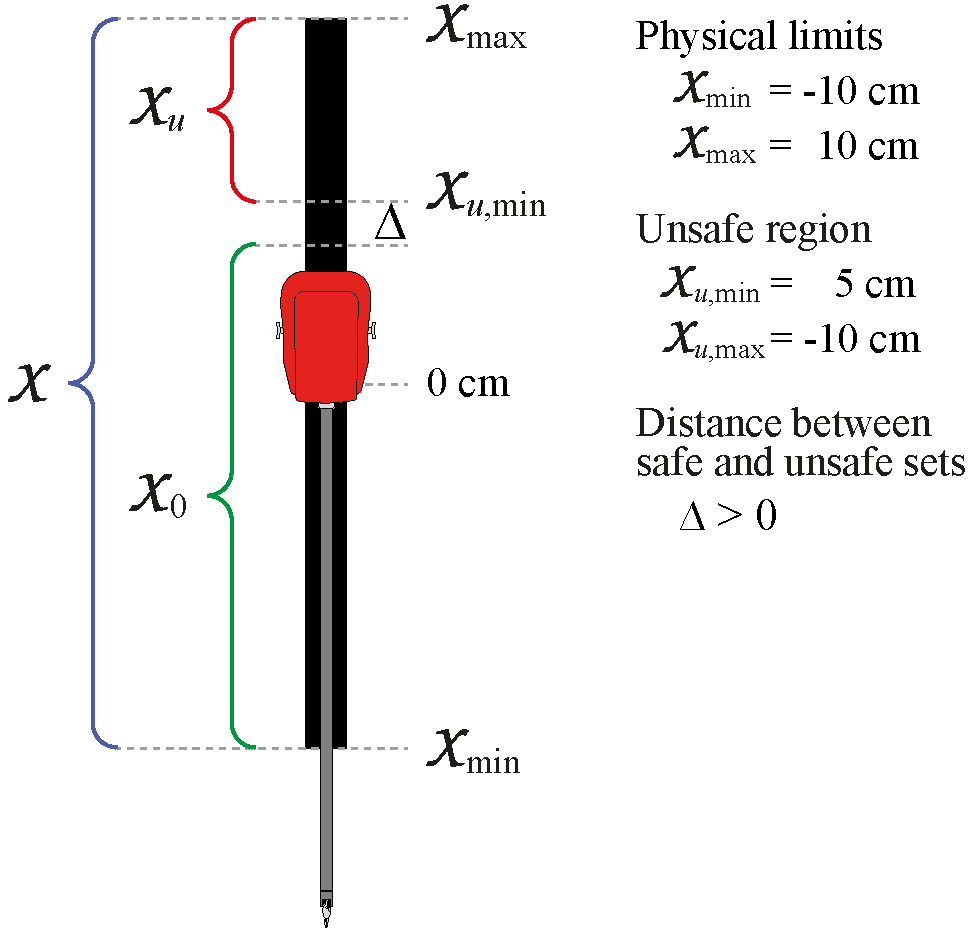
\includegraphics[width=0.42\textwidth]{slide_sos.pdf}
\caption{The boundaries in slide position of the robotic instrument for each of the sets $\mathcal{X}$, $\mathcal{X}_u$ and $\mathcal{X}_0$,  is visualized for the instrument house.}
	\label{fig:sos_slide}
\end{figure}

Using the first order linear model of the robot slide system described in \autoref{subsec:model_1d}, and  the linear position controller described in \autoref{sec:K_Nbar_1D_1storder} with proportional gain \textbf{K} and unity gain between reference and position secured by $\bar{\mathbf{N}}=\textbf{K}+1$, %giving input $u=\bar{\mathbf{N}}x_\text{ref}-\textbf{K}x$, 
the closed-loop system is recapitulated as
%i.e. for the  1D state space system with $x_1\in\mathcal{X}\subset\mathbb{R}$ corresponding to the robot slide joint being the only degree of freedom (see \autoref{fig:safe:overview} for an overview of the slide movement), thus a closed-loop system
\vspace{-1mm}
\begin{align}
\dot{x}_1 = \textbf{A}x_1+\textbf{B}u &= \textbf{A}x_1+\textbf{B}(\bar{\mathbf{N}}x_\text{ref}-\textbf{K}x_1)\nonumber\\
&= \underbrace{(\textbf{A} - \textbf{B}\textbf{K})}_{-\tau^{-1}(\textbf{K}+1)} x_1 + \underbrace{\textbf{B}\bar{\textbf{N}}}_{\tau^{-1}(\textbf{K}+1)} x_\text{ref} \nonumber\\
& = %-\tau^{-1}x+\tau^{-1}u=
%-\tau^{-1}x+\tau^{-1}(\bar{\mathbf{N}}x_\text{ref}-\textbf{K}x), 
\tau^{-1}(\mathbf{K}+1)(x_\text{ref}-x_1),
\kk\kk\mm \text{with }\tau=110\,\text{ms}\label{eq:sos_firstorder}
\end{align}


This system is used in the following subsections in the barrier function search.
First with a reference in zero giving detailed explanations of the program formulation, and subsequently for the same system, testing for how wide a range of references safety can be guaranteed. Last, a coordinate shift from the position-reference-space to the error-space is performed in order to simplify the search for reference intervals yielding valid solutions.

\subsection{Safety Verification of First Order System with Zero Reference}\label{subsec:zeroref}
To give a clear picture of the structure of the \gls{sos} program, an initial exhaustive example is given for the  one-dimensional first order system with zero as reference position. Commands associated with SOSTOOLS is marked in brown in the following code snips. The full code can be found in \autoref{app:sos_noref} and on the attached cd on the path \texttt{matlab\_scripts/sostools/1storder\_noRef.m}

Search for a barrier certificate by first defining the open-loop system, and designing a controller (with pole placement) as described in \autoref{sec:K_Nbar_1D_1storder}.
\begin{lstlisting}[language=matlab]
% Time constant from measurement
tau = 0.11;
% State-space matrices from first order system
A = -1/tau;
B = 1/tau;
K = place(A,B,10*eig(A));
\end{lstlisting}
%Define the boundaries for each of the three sets $\mathcal{X}$, $\mathcal{X}_u$ and $\mathcal{X}_0$ as given in \autoref{fig:slide_sos}, and 
Define the desired distance $\Delta$ between the safe and unsafe sets along with  the minimum value $\bar{\epsilon}$ of the barrier function on the unsafe set. %in order to get $\mathcal{X} =\{x\in[-0.1,0.1]\}$, $\mathcal{X}_u=\{x\in[0.05,0.1]\}$ and $\mathcal{X}_0=\{x\in[-0.1,0.05-\Delta]\}$.
\begin{lstlisting}[language=matlab]
% Distance between defined safe and unsafe regions
delta = 1e-3;

% Minimum value of the barrier certificate on the unsafe set Xu
epsilon = 1e-3;
\end{lstlisting}
%% Set upper and lower limits for the set intervals X, Xu and X0
%Xmax = 0.1;
%Xmin = -0.1;
%Xumax = Xmax;
%Xumin = 0.05;
%X0max = Xumin-delta;
%X0min = Xmin;
%\end{lstlisting}

Then the symbolic state variables are declared for the SOS program in SOSTOOLS with the command \texttt{pvar}. % (which corresponds to the command \texttt{syms} in the MATLAB symbolic toolbox). 
Now the SOS program \texttt{prog} can be initialized using the function \texttt{sosprogram} which takes the state variable as input. 
\begin{lstlisting}[language=matlab]
% Declare state variables
pvar x1

% Initialize the sum of squares program
prog = sosprogram(x1);
\end{lstlisting}
%The reference for the robot position is generated as the 1D heart position, taking into account the system gain $\bar{N}$, and the closed-loop system equation is written as a function of the sybolic state. %\textcolor{red}{Something is wrong with the reference..?}
The vector field or derivative of the state can now be defined in terms on the symbolic state variable. This function is necessary for the SOS program when requiring that the Lie derivative of the barrier certificate must be negative on the set $\mathcal{X}$.
\begin{lstlisting}[language=matlab]
% Vector field dx/dt = fx (closed loop)
fx = (A-B*K)*x1;
\end{lstlisting}
For ease of defining a (1D) function $g$ that is positive on an interval [$p_1, p_2$], a parabola function is used.
\begin{lstlisting}[language=matlab]
function [a,b,c] = parabola(p1,p2,a)
	if ~exist('a','var')
		a=-1;
	end
	b=a*(p1^2-p2^2)/(p2-p1);
	c=-a*p1^2-b*p1;
end
\end{lstlisting}
Now declare the polynomial barrier function with the command \texttt{sospolyvar}. To do this, a monomial vector must be specified with \texttt{monomials} (see the monomial example in \autoref{eq:monomial_example}), which takes the state variable and the monomial degree(s) as input. The monomial degrees for $B(x_1)$ are chosen as low as possible until a solution can be found. In this case a solution can be found for a degree of $B(x_1)$ that is [0:4], i.e. a polynomial in $x_1$ of degrees zero through four.
\begin{lstlisting}[language=matlab]
% Declare the polynomial barrier function
zB = monomials(x1,0:4);
[prog,Bar] = sospolyvar(prog,zB);
\end{lstlisting}
Now the set $\mathcal{X}$ can be defined as the slide region according to \autoref{fig:sos_slide} using the Lie derivative inequality in \autoref{cer3_putinar}, which is defined with the command \texttt{sosineq}. The SOS polynomials $q$ are of the form in \autoref{eq:sos_polynomial}, i.e. $q=\mathbf{z}^T\mathbf{Q}\,\mathbf{z}$ (so the degree of $q$ is twice the degree of the monomial vector $\mathbf{z}$), and are declared with the command \texttt{sossosvar}, also taking a monomial vector as input.
\begin{lstlisting}[language=matlab]
% Define space X in Rn
[a,b,c] = parabola(-0.1,0.1); % get coefficients for parabola which is positive for x in [-0.1,0.1] m
gX = a*x1^2+b*x1+c;

zX = monomials(x1,0:4);
[prog,qX] = sossosvar(prog,zX);

prog = sosineq(prog,-diff(Bar,x1)*fx-gX*qX);
\end{lstlisting}
Similarly, the unsafe region $\mathcal{X}_u$ is defined according to the SOS inequality in \autoref{cer2_putinar} as the area between slide positions 5-10\,cm as given by \autoref{fig:sos_slide}.
\begin{lstlisting}[language=matlab]
% Define space Xu in X
[a,b,c]=parabola(0.05,0.1);
gXu = a*x1^2+b*x1+c;

zXu = monomials(x1,0:4);
[prog,qXu] = sossosvar(prog,zXu);

prog = sosineq(prog,Bar-epsilon-gXu*qXu);
\end{lstlisting}
And finally the region $\mathcal{X}_0$ is defined according to the SOS inequality in \autoref{cer1_putinar} as $\mathcal{X}_0\subset\mathcal{X}\setminus\mathcal{X}_u$, separated from the unsafe set by the distance $\Delta$.
\begin{lstlisting}[language=matlab]
% Define space X0 in X
[a,b,c]=parabola(-0.1,0.05-delta);
gX0 = a*x1^2+b*x1+c;

zX0 = monomials(x1,0:4);
[prog,qX0] = sossosvar(prog,zX0);

prog = sosineq(prog,-Bar-gX0*qX0);
\end{lstlisting}
With all three areas defined according to \autoref{def:barrier_sos}, the program is ready to be solved by using the command \texttt{sossolve}. If a solution is found, an overview of the solution accuracy is printed in the MATLAB terminal as the residual norm, feasibility ratio, number of iteration steps and solving time. To get the polynomial $B(x_1)$ use the function \texttt{sosgetsol}.
\begin{lstlisting}[language=matlab]
% Solve for barrier certificate
prog = sossolve(prog);
getB = sosgetsol(prog,Bar)
\end{lstlisting}

\vspace{-2mm}
From the terminal printout it is verified that the problem is neiter primal or dual infeasible, and that the feasibility ratio for this solution is given as 1.0122, which is fairly close to 1 and hence indicates that the solution is valid. The solution is found in 15 iterations with a residual norm of 7.5521e-10 and thereby no indication of numerical errors.

To additionally verify that the solution is indeed valid, it is tested that the solution complies with the inequalities being \gls{sos} by testing if they can be resolved to the form in \autoref{eq:sos_polynomial}.
\begin{lstlisting}[language=matlab]
% Get coefficients for the remaining polynomials
getdBdx = diff(getB,x1)
getqXu1 = sosgetsol(prog,qXu);
getqX01 = sosgetsol(prog,qX0);
getqX1 = sosgetsol(prog,qX);

% Test if the inequalities are SOS
[Q,~,~] = findsos(getB-epsilon-gXu*getqXu1);
[Q2,~,~] = findsos(-getB-gX0*getqX01);
[Q3,~,~] = findsos(-detdBdx*fx-gX*getqX1);
\end{lstlisting}
%Result
%\begin{lstlisting}[language=matlab]
%Size: 188   33
%
%SeDuMi 1.3 by AdvOL, 2005-2008 and Jos F. Sturm, 1998-2003.
%Alg = 2: xz-corrector, Adaptive Step-Differentiation, theta = 0.250, beta = 0.500
%Put 5 free variables in a quadratic cone
%eqs m = 33, order n = 36, dim = 190, blocks = 8
%nnz(A) = 197 + 0, nnz(ADA) = 493, nnz(L) = 263
%it :     b*y       gap    delta  rate   t/tP*  t/tD*   feas cg cg  prec
%0 :            9.49E-01 0.000
%1 :   9.95E-04 1.03E-02 0.000 0.0109 0.9990 0.9990   1.00  1  1  5.3E-02
%2 :   1.92E-03 2.95E-03 0.000 0.2857 0.9000 0.9000   0.77  1  1  1.9E-02
%3 :   9.73E-03 7.23E-04 0.000 0.2453 0.9000 0.9000  -0.07  1  1  1.4E-02
%4 :   1.64E-01 6.45E-05 0.000 0.0892 0.9900 0.9900  -0.83  1  1  1.7E-02
%5 :   7.57E-01 1.66E-05 0.000 0.2580 0.9000 0.9000  -1.02  1  1  2.0E-02
%6 :   3.17E+00 4.40E-06 0.000 0.2641 0.9000 0.9000  -1.09  3  3  2.0E-02
%7 :   8.00E+00 1.35E-06 0.000 0.3071 0.9038 0.9000  -0.91  1  2  1.8E-02
%8 :   1.16E+01 3.80E-07 0.000 0.2815 0.9132 0.9000  -0.61  2  2  1.1E-02
%9 :   8.37E+00 8.48E-08 0.000 0.2232 0.9000 0.9067   0.05  2  2  3.9E-03
%10 :   4.64E+00 1.41E-08 0.000 0.1661 0.9056 0.9000   0.13  3  3  1.1E-03
%11 :   1.34E+00 2.89E-09 0.000 0.2049 0.9088 0.9000   0.77  4  3  2.6E-04
%12 :   7.91E-02 1.99E-10 0.436 0.0688 0.9900 0.9901   0.91  4  4  1.9E-05
%13 :   7.47E-03 1.24E-11 0.473 0.0624 0.9907 0.9900   0.94  4  4  1.3E-06
%14 :   2.91E-04 5.14E-13 0.486 0.0414 0.9900 0.9900   0.99  4  4  5.5E-08
%15 :   3.18E-06 1.10E-14 0.223 0.0215 0.9900 0.9905   1.01  5  5  1.1E-09
%
%iter seconds digits       c*x               b*y
%15      0.4   7.4  0.0000000000e+00  3.1754678011e-06
%|Ax-b| =   7.6e-10, [Ay-c]_+ =   2.3E-10, |x|=  1.7e+05, |y|=  8.0e+04
%
%Detailed timing (sec)
%Pre          IPM          Post
%6.200E-02    3.130E-01    2.300E-02    
%Max-norms: ||b||=1.000000e-03, ||c|| = 0,
%Cholesky |add|=1, |skip| = 0, ||L.L|| = 9.42104e+12.
%
%Residual norm: 7.5521e-10
%
%iter: 15
%feasratio: 1.0122
%pinf: 0
%dinf: 0
%numerr: 0
%timing: [0.0620 0.3130 0.0230]
%wallsec: 0.3980
%cpusec: 0.4531
%
%
%getB = 
%373.0249*x1^4 + 151.3339*x1^3 + 16.8843*x1^2 - 6.4509e-06*x1 - 0.061301
%
%
%getdBdx = 
%1492.0996*x1^3 + 454.0017*x1^2 + 33.7686*x1 - 6.4509e-06
%\end{lstlisting}

\vspace{-5mm}
This is indeed the case, and it is thereby verified that a barrier certificate is found for the closed-loop system in \autoref{eq:sos_firstorder}, namely
\vspace{-2mm}
\begin{equation}
B(x_1) = 373.0249\cdot x_1^4 + 151.3339\cdot x_1^3 + 16.8843\cdot x_1^2 - 6.4509e\text{-}6\cdot x_1 - 0.061301
\end{equation}

\vspace{-3mm}
The first three coefficients of the polynomial barrier certificate are of ample size (not in the order 1e-5 or less), while the fourth seem unimportant. Decreasing the degree of the monomial $\mathbf{z}_B$ (and thereby\,the\,order of $B$) to [0,2:4] %does, however, not prove a proper solution, as the inequality \autoref{cer3_putinar} cannot be resolved on the form in \autoref{eq:sos_polynomial} and hence is not \gls{sos}. 
gives the solution
\begin{equation}
B(x_1) = 290.559\cdot x_1^4 + 112.4642\cdot x_1^3 + 12.2165\cdot x_1^2 - 0.044304
\end{equation}
which is also a valid barrier certificate, found in 13 iterations with feasibility ratio 0.9797 and a residual norm of 1.0412e-09.
The two barrier certificates are depicted in \autoref{fig:1D_1stordersys_noRef}, from which it is seen that  both comply with the requirements for a barrier certificate, i.e. they are positive ($B(x_1)\geq \bar{\epsilon}$) on $\mathcal{X}_u=\{x_1\in [0.05,0.1]\}$ and negative on $\mathcal{X}_0=\{x_1\in [-0.1,0.05-\Delta]\}$, and their Lie derivatives are nonpositive on $\mathcal{X}=\{x_1\in [-0.1,0.1]\}$, in accordance with \autoref{def:barrier_certificate}. It is also seen that the value of each of the barrier certificates on the set $\mathcal{X}$ seem reasonable being neither exceptionally small or large, verifying that the choice of $\bar{\epsilon}$ seems reasonable.

\begin{figure}[htbp]
\centering%	\hspace*{-12mm}
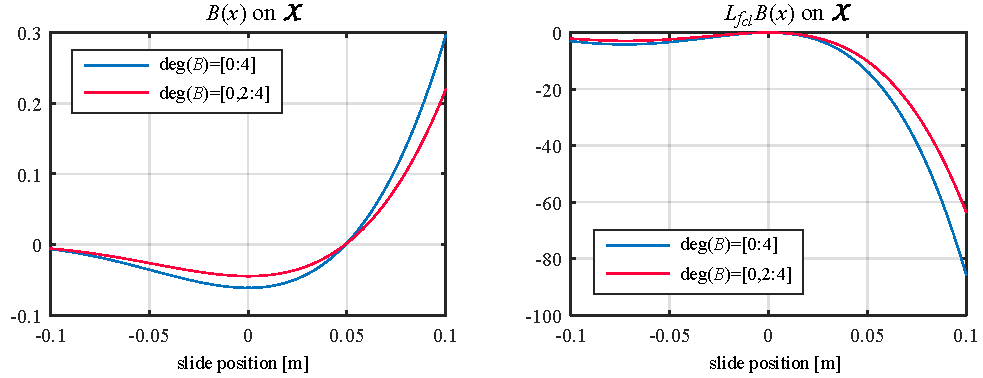
\includegraphics[width=0.9\textwidth]{1D_1stordersys_noRef.pdf}
	\caption{Barrier certificates found with SOSTOOLS for the first order system in \autoref{eq:sos_firstorder} with zero reference,  that comply with the requirements in \autoref{def:barrier_sos}. }
	\label{fig:1D_1stordersys_noRef}
\end{figure}

It is noted that the safety verification is accomplished with a fourth order polynomial barrier certificate, while it can be argued that it could be possible with a second order polynomial. This is, however, not important for the safety verification of the system, where the conclusion is that a solution can be found, thus the system is safe.










\subsection{Verifying a Range of Reference Positions for the First Order System}\label{sec:sos_1storder_references}

\vspace{-2mm}
Now a non-zero reference is introduced. As it is desired to verify safety for a whole range of references, the barrier polynomial is now formulated as a function of both position and reference $B(x,x_\text{ref})$, thus introducing the reference as an independent state implying an augmented state space equation equivalent to \autoref{eq:sos_firstorder}: 
%However, from \autoref{eq:sos_firstorder} it can be seen that with the unity gain matrix $\bar{\mathbf{N}}$ the system can be  written as
\begin{equation}
\dot{\mathbf{x}}=\dot{\begin{bmatrix}
x_1\\x_\text{ref}
\end{bmatrix}} 
= \begin{bmatrix}
\mathbf{A}+\textbf{BK} & \textbf{B}\bar{\mathbf{N}}\\
0 & 0
\end{bmatrix}
\begin{bmatrix}
x_1\\x_\text{ref}
\end{bmatrix}
= \begin{bmatrix}
-\tau^{-1}(\mathbf{K}+1) & \tau^{-1}(\mathbf{K}+1)\\
0 & 0
\end{bmatrix}
\begin{bmatrix}
x_1\\x_\text{ref}
\end{bmatrix}
\label{eq:1storder_augmented}
\end{equation}

In the \gls{sos} program constraints are set up for the new variable \texttt{xref}  for each of the sets, included as extra terms in the sums in \autoref{def:barrier_sos}, e.g. for the set $\mathcal{X}$ a new term with \gls{sos} polynomial $q(\mathbf{x})$ and polynomial $g(x_\text{ref})$, positive on the  reference  interval \texttt{[rMin,rMax]}, is included in the inequality as:
\begin{lstlisting}[language=matlab]
% Constraint on the set X being nonpositive for the interval of references 
[a,b,c] = parabola(rMin,rMax); 
gX2 = a*xref^2+b*xref+c;

zX2 = monomials([x1,xref],0:2);
[prog,qX2] = sossosvar(prog,zX2);

prog = sosineq(prog,-[diff(Bar,x1) diff(Bar,xref)]*[fx;0] - gX1*qX1 - gX2*qX2);
\end{lstlisting}

The goal is to verify safety of this system for a range of references, preferably for all references within the safe position interval, such that the sets would be as depicted in \autoref{fig:sos_Xregion}.

\subsubsection{Expected Barrier Certificate Geometry}

\vspace{-2mm}
In order to get a picture of the expected outcome, a brief analysis of the considered state space is made.
It can be seen from \autoref{eq:1storder_augmented} that the system vector field will be zero when $x_1=x_\text{ref}$, which in turn means that the Lie derivative of the barrier function will be zero for $x_1=x_\text{ref}$, marked in \autoref{fig:sos_Xregion_dBdx} with a green line. 
To the upper left of this line the system will have a positive time derivative, thus requiring that the derivative of the barrier function with respect to $x_1$ must be negative in this region in order to comply with \autoref{cer3} i.e. $L_{f_{cl}}B(\mathbf{x}) \leq 0$. 
Thus, to the left of this line the barrier polynomial will have decreasing values in the positive $x_1$ direction. 
\begin{figure}[htbp]
	\centering
	\subbottom[]{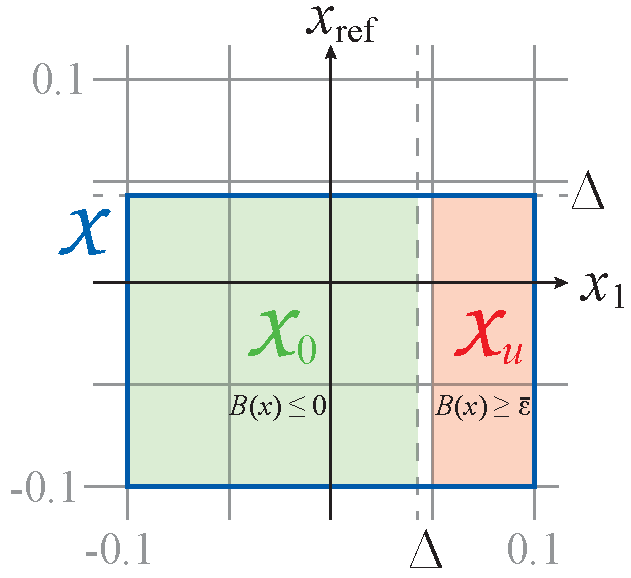
\includegraphics[width=0.3\textwidth]{sos_Xregion.pdf}\label{fig:sos_Xregion}}%
	\hspace{3mm}
	\subbottom[]{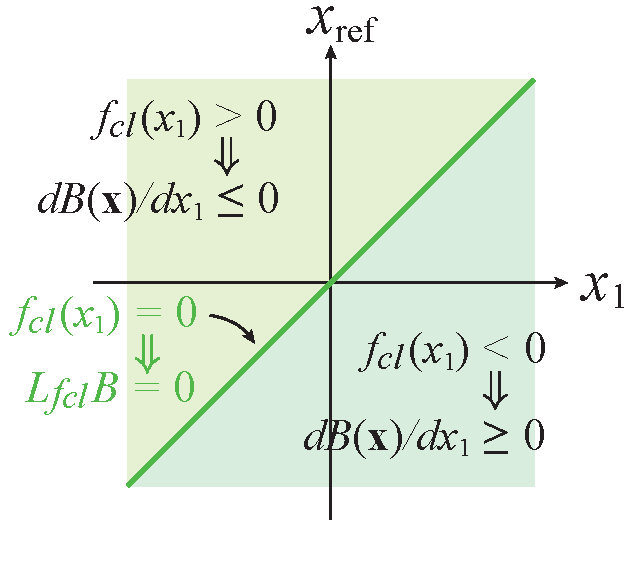
\includegraphics[width=0.3\textwidth]{sos_Xregion_dBdx.pdf}\label{fig:sos_Xregion_dBdx}}%
	\hspace{3mm}
	\subbottom[]{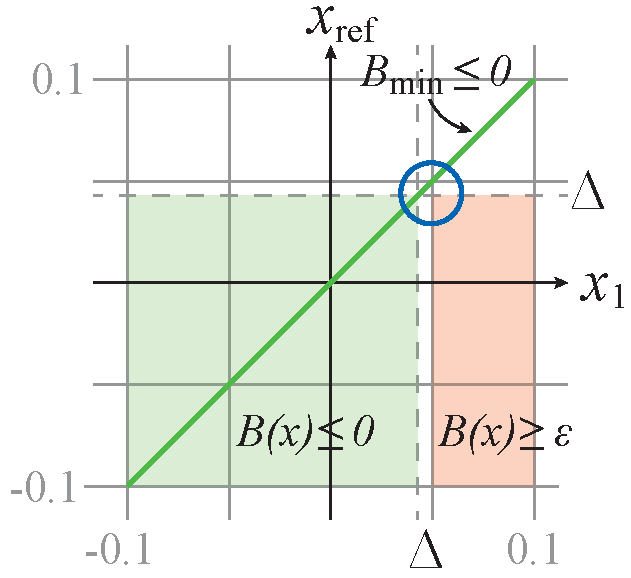
\includegraphics[width=0.3\textwidth]{sos_Xregion_Bvalue.pdf}\label{fig:sos_Xregion_Bvalue}}%
	\caption{Outline of the safe and unsafe sets marking the value requirements for the barrier certificate as a function of the robot position and the  position reference. % \Autoref{fig:sos_Xregion} depicts a set $\mathcal{X}$ where all references within the safe positions are allowed.
		\Autoref{fig:sos_Xregion_dBdx} sketches that $L_{f_{cl}}B(\mathbf{x})=0$  in $x_1=x_\text{ref}$ as inferred from \autoref{eq:sos_firstorder}. %, and \autoref{fig:sos_Xregion_Bvalue} shows a zero level set for $B(x)$.
	}
	\label{fig:sets_reference}
\end{figure}
To the lower right of the green line the system will have negative time derivative, thus analogously requiring that the derivative $dB/dx_1$ must be positive in this region, meaning that $B(\mathbf{x})$ will have increasing values in the positive $x_1$ direction here.
%Requiring a zero level set of the barrier certificate between $x_1=0.05-\Delta$ and $x_1=0.05$, this means that the value of $B(x)$ \textcolor{red}{something something}

In \autoref{fig:sos_Xregion_Bvalue} the zero level set of a barrier function is sketched with a red line between the safe and unsafe regions. As this level set gets  closer to the green line indicating the zero-value of the Lie derivative for increasing values of $x_\text{ref}$, it is expected that the value of  $B(\mathbf{x})$ is increasing along this line in the positive $x_\text{ref}$ direction.

%As this line crosses through the safe region, it means that it will be a minimum value of the barrier function of negative value. In \autoref{fig:sos_Xregion_Bvalue} it can be seen that this minimum is very close to the zero level set around the unsafe region, requiring a very high degree polynomial to obtain this shape of zero level set. This can be resolved by decreasing the upper value of allowed references, as illustrated in \autoref{fig:sos_Xregion_Bvalue_limitref} with an example of a fairly smooth zero level set.



\subsubsection{Results and Conclusions}

\vspace{-2mm}
A number of tests are run with SOSTOOLS varying the values of the parameters  $\bar{\epsilon}$, $\Delta$, and the degree of the \gls{sos} polynomials $q_j$ and the polynomial $B(\mathbf{x})$, % itself, in order to understand the effect of varying each of these parameters and to test for which intervals of references a solution can be found.
%A solution found with SOSTOOLS is considered valid if it passes the test that each of the expressions in the inequalities are \gls{sos} by testing if they can be resolved on the form in \autoref{eq:sos_polynomial}. The analysis in the following is based on the results for these solutions, with 
in order to see for how high a level of the upper  end  of the allowed reference interval, \texttt{rMax}, solutions can be found. The MATLAB implementation can be found in appendix \ref{app:sos_refinterval} and in \autoref{app:cd} under the path \texttt{matlab\_scripts/sostools/1storder\_withRef.m}.
As seen from \autoref{fig:sets_reference} $\bar{\epsilon}$ is the minimum value of the barrier function on the unsafe set, and increasing this may require the zero level set to be pushed further away from $\mathcal{X}_u$. This may in turn require also increasing the distance $\Delta$ to the safe set, i.e. contracting the region $\mathcal{X}_0$.
The conclusions are summarized in \autoref{tab:sostools_varying_param}.


%It makes sense that increasing epsilon will also require a slight increase in delta from the figure, as the zero level set of B has to be between the two sets i.e. decreasing the region X0.

\begin{table}[htbp]
\begin{tabularx}{\textwidth}{l X}
\rowcolor{HeaderBlue}
\textbf{Parameter} & \textbf{Effect of variation}\\
deg$(B)$ & In general the feasibility ratio is better (closer to one) when testing for higher degrees of $B(\mathbf{x})$ ([0:6] or [0:8] compared to [0:4]), and solutions can be found for larger intervals of the reference when $B(\mathbf{x})$ has higher degree.\\
\rowcolor{textBlue}
deg$(q_j)$ & Increasing the degree of the \gls{sos} polynomials (monomial degrees [0:6] compared to [0:2] or [0:4]) generally degrades the feasibility ratio.\\
$\bar{\epsilon}$ & Increasing $\bar{\epsilon}$ decreases the allowed reference interval and also shows a trend of slightly increasing the residual norm. Increasing $\bar{\epsilon}$ iteratively proves that gradually an increase in $\Delta$ is also required in order for solutions to be found. \\
\rowcolor{textBlue}
$\Delta$ & Generally increasing $\Delta$ will also decrease the allowed interval of references, and shows a trend of decreasing the residual norm until some limit.\\
\textbf{K} & Lowering the gain of the controller increases  the allowed reference interval.
\end{tabularx}
\caption{Effect of varying different parameters in the \gls{sos} program; see \autoref{fig:sos_delta1} for a visualization of $\bar{\epsilon}$ and $\Delta$. Results are only included for solutions where all inequalities were verified to be \gls{sos} with \texttt{findsos}.}
\label{tab:sostools_varying_param}
\end{table}

Numerical problems are reported for all solutions found, and the residual norms (size of numerical error in the solution) are in general in the order of -3 and -4, so it is desired to keep the degree of polynomials low and to increase the value of $\bar{\epsilon}$, compared to \autoref{subsec:zeroref} to be sure that the numerical error of the solution does not cause the barrier polynomial to attain nonpositive values on the unsafe set. 

%Point of departure is taken in the same values for the parameters $\bar{\epsilon}$ and $\Delta$, and degrees of the \gls{sos} polynomials $q_j$ and the barrier certificate as presented in \autoref{subsec:zeroref}, i.e. $\bar{\epsilon}=0.001$, $\Delta=0.001$, deg$(B)=$[0:4] and all \gls{sos} polynomials deg$(q_j)=$[0:4]. The same controller gain is used as described in \autoref{sec:K_Nbar_1D_1storder} ($\textbf{K}=9$), and a small interval of references around zero is used initially.

%The interval of references for which a solution can be found depends on all of the parameters summarized in \autoref{tab:sostools_varying_param}. The lower limit of allowed references in $\mathcal{X}_0$ is independent of the parameters, though,  as no irrealizable requirements are set for $B(x)$ in this region. 



%This obviously comes at the cost of a somewhat more lengthy polynomial expression, the fourth order polynomial given as (decimals are left out for clarity)
%\begin{align}
%%B4_q4 Residual norm: 0.00060655 feasratio: 0.7455 numerr: 0
%B(\textbf{x}) = \,\,\,\,\,&
%2608 x_1^4 - 2292 x_1^3 x_\text{ref} - 1441 x_1^2 x_\text{ref}^2 - 625
% x_1 x_\text{ref}^3 - 3 x_\text{ref}^4 
% + 625 x_1^3 - 811 x_1^2 x_\text{ref} \nonumber\\
%&- 244 x_1 x_\text{ref}^2 + 25 x_\text{ref}^3 + 43 x_1^2 
%- 86 x_1 x_\text{ref} 
%+ 14 x_\text{ref}^2 + 0.005 x_1 + 6 x_\text{ref} - 0.2\label{eq:B4_q4_e0001}
%\end{align}
%and the sixth order polynomial expression as\\ 
%
%\textcolor{white}{phantom}
%\vspace{-10mm}
%\begin{align}
%%B6_q4 Residual norm: 0.00087217 feasratio: 0.6538 numerr: 0
%B(\mathbf{x}) = \,\,\,\,\,& 
%8959  x_1^6 + 4709  x_1^5x_\text{ref} - 1937 x_1^4 x_\text{ref}^2 - 10924   x_1^3  x_\text{ref}^3 - 9569  x_1^2  x_\text{ref}^4 - 7611  x_1  x_\text{ref}^5 - 6662  x_\text{ref}^6 \nonumber\\
%&+ 16569  x_1^5 - 9805  x_1^4  x_\text{ref} - 6751  x_1^3  x_\text{ref}^2 
%- 12699  x_1^2  x_\text{ref}^3 + 5592  x_1  x_\text{ref}^4 - 4094  x_\text{ref}^5 
%+ 9420  x_1^4 \nonumber\\
%&- 15027  x_1^3  x_\text{ref} + 7407  x_1^2  x_\text{ref}^2 
%- 6938  x_1  x_\text{ref}^3 - 1421  x_\text{ref}^4 + 1409  x_1^3 - 2717  x_1^2
%  x_\text{ref} + 1233  x_1  x_\text{ref}^2 \nonumber\\
%& + 244 x_\text{ref}^3 + 73  x_1^2 - 146
%  x_1  x_\text{ref} - 84  x_\text{ref}^2 - 0.002  x_1 + 15  x_\text{ref} - 0.412\label{eq:B6_q4_e0001}
%\end{align}

The choice of parameter values are explained in \autoref{tab:sostools_choice} and the barrier certificate is plotted in \autoref{fig:1storder_withRef} separately for the safe and unsafe sets to validate the sign of $B(\mathbf{x})$ on each set. 
Evaluating the curve for the barrier polynomial and its Lie derivative,  the geometric considerations are verified in that $B(\mathbf{x})$ indeed is (slightly) decreasing along the $x_1$ axis to the left of the line $x_1=x_\text{ref}$, and increasing to the right, as seen on the plot of $\mathcal{X}_0$ (and increasing along the $x_1$ axis on the entire set $\mathcal{X}_u$). It is also verified that the Lie derivative is zero along the line $x_1=x_\text{ref}$. Thereby it is verified that the barrier certificate is valid according to \autoref{def:barrier_certificate},  guaranteeing  safety for the first order system in \autoref{eq:1storder_augmented} with references in the interval $x_\text{ref}\in [\texttt{rMin,rMax}]=[-0.1,0.017]$\,m.



\begin{table}[H]
	\begin{tabularx}{\textwidth}{l X}
		\rowcolor{HeaderBlue}
		\textbf{Choice} & \textbf{Reason}\\
		deg$(B)=$ [0:6] & Increasing the degree of $B(\mathbf{x})$ from [0:4] to [0:6] elevates the upper limit for allowed references. Increasing the degree (keeping the remaining parameters constant) yields an infeasible solution. \\
		\rowcolor{textBlue}
		deg$(q_j)=$ [0:2] & Keeping the degree low, as increased degree entails poorer feasibility ratio and greater residual norm.\\
		$\bar{\epsilon}=0.1$ & Smaller values of  $\bar{\epsilon}$ allows solutions to be found for larger values of \texttt{rMax}, while the residual norm  speaks in favour of increasing $\bar{\epsilon}$. A compromise is made, as this choice of $\bar{\epsilon}$ gives a residual norm that is approximately twice as big as with $\bar{\epsilon}=0.01$, while it is almost an order of magnitude smaller than for $\bar{\epsilon}=1$.\\
		\rowcolor{textBlue}
		$\Delta=0.015$ & It is preferred to have as small a value of $\Delta$ as possible, as this increases the value of \texttt{rMax} for which solutions can be found. On the other hand lower  values of $\Delta$ deteriorate the feasibility ratio. The value is increased slightly along with $\bar{\epsilon}$ until a solution is found. \\
		$\textbf{K}=0.2$ & Lower gain allows a larger value of \texttt{rMax} (the demand $L_{f_{cl}}B(\textbf{x}) \leq 0$ is affected by $\textbf{K}$), and it is known from the implementation described in \autoref{sec:davinci-implementation}, that at present time the controller gain implemented is approximately this size.
	\end{tabularx}
	\caption{Chosen value for each of the parameters. The barrier certificate is plotted in \autoref{fig:1storder_withRef}.}
	\label{tab:sostools_choice}
\end{table}


%Generally increasing $\Delta$ will also decrease the allowed interval and shows a trend of decreasing the residual norm until some limit where it doesn't seem to affect the construction of B so much more.

%\begin{figure}[H]
%\centering
%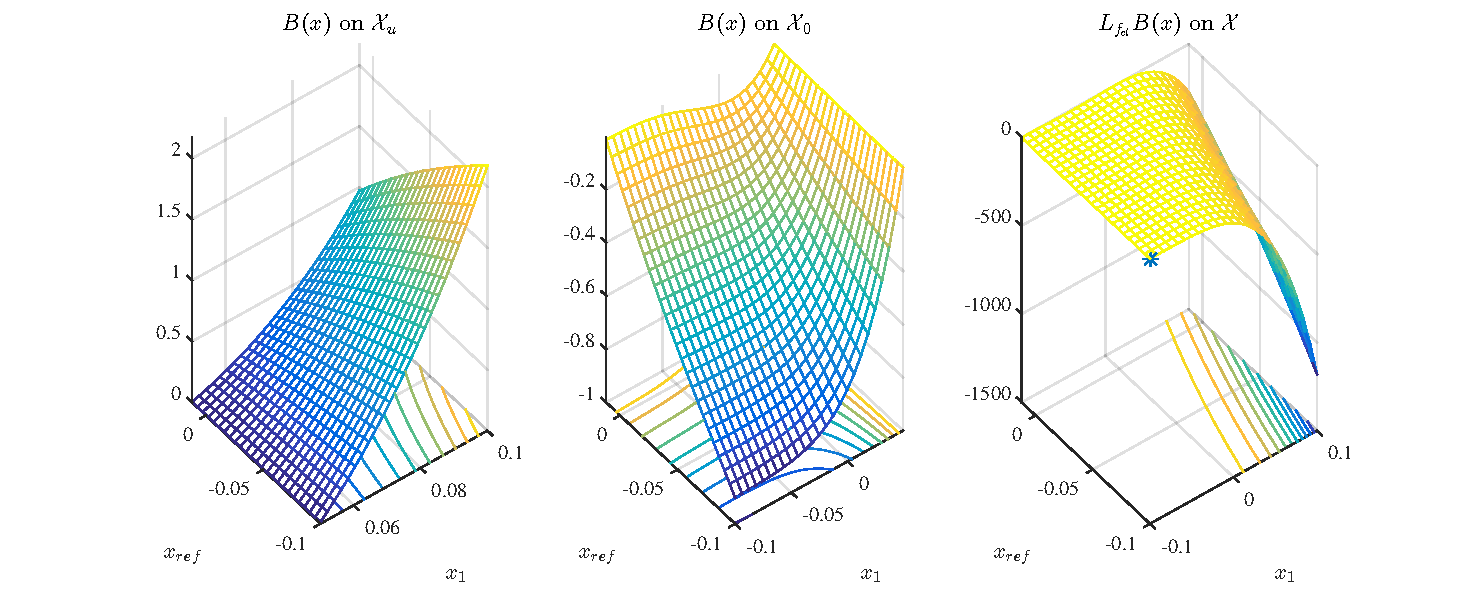
\includegraphics[width=\textwidth]{1D_1stordersys_withRef_k9_B4_q4.pdf}
%\caption{Barrier certificate of degree [0:4], all \gls{sos} polynomials of degree [0:4], $\bar{\epsilon}=0.001$, $\Delta=0.001$ and gain $\textbf{K}=9$ allows an interval of references [-0.1,0.012], with \texttt{feasratio=0.7455} and \texttt{Residual norm=6.1e-4}.}
%\label{fig:1D_1stordersys_withRef_k9_B4_q4}
%\end{figure}
%\vspace{2mm}
%\begin{figure}[H]
%\centering
%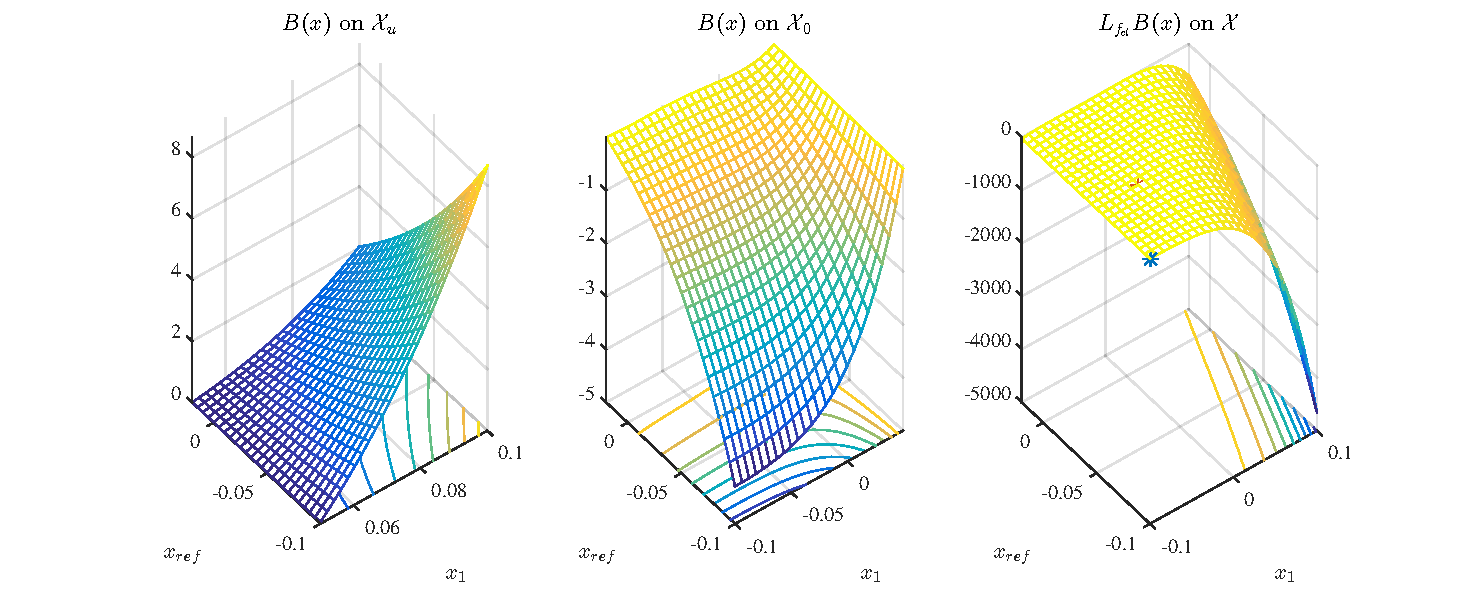
\includegraphics[width=\textwidth]{1D_1stordersys_withRef_k9_B6_q4.pdf}
%\caption{Barrier certificate of degree [0:6], all \gls{sos} polynomials of degree [0:4], $\bar{\epsilon}=0.001$, $\Delta=0.001$ and gain $\textbf{K}=9$ allows an interval of references [-0.1,0.02], with \texttt{feasratio=0.6538} and \texttt{Residual norm=8.7e-4}.}
%\label{fig:1D_1stordersys_withRef_k9_B6_q4}
%\end{figure}


%The asterisks in each of the plots of $L_{f_{cl}}B(x)$ marks spots on the curve where its value is positive, which in all cases happen along the line $x_1=x_\text{ref}$. The reason for this error is the numerical problems encountered for all of the solutions.

%\Autoref{fig:1D_1stordersys_withRef_k02_B6_q2} shows a plot of another sixth order polynomial barrier certificate found for a system with feedback gain $\mathbf{K}=0.2$, which is valid for references in an interval extending up to 3.2\,cm.

%\vspace{5mm}
%\begin{figure}[htbp]
%\centering
%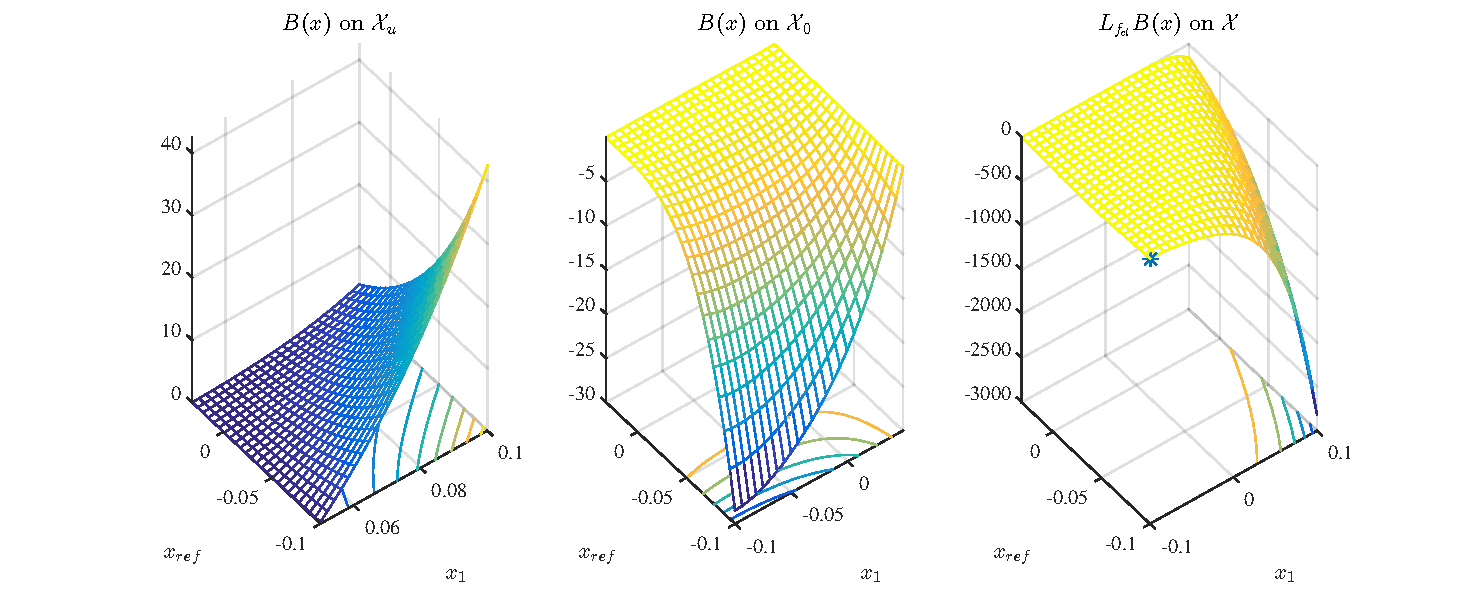
\includegraphics[width=\textwidth]{1D_1stordersys_withRef_k02_B6_q2.pdf}
%\caption{Barrier certificate of degree [0:6], all \gls{sos} polynomials of degree [0:2], $\bar{\epsilon}=0.001$, $\Delta=0.001$ and gain $\textbf{K}=0.2$ allows an interval of references [-0.1,0.032], with \texttt{feasratio=0.5349} and \texttt{Residual norm=8.1e-4}.}
%\label{fig:1D_1stordersys_withRef_k02_B6_q2}
%\end{figure}
%\vspace{5mm}




\vspace{-2mm}
\begin{figure}[H]
\centering
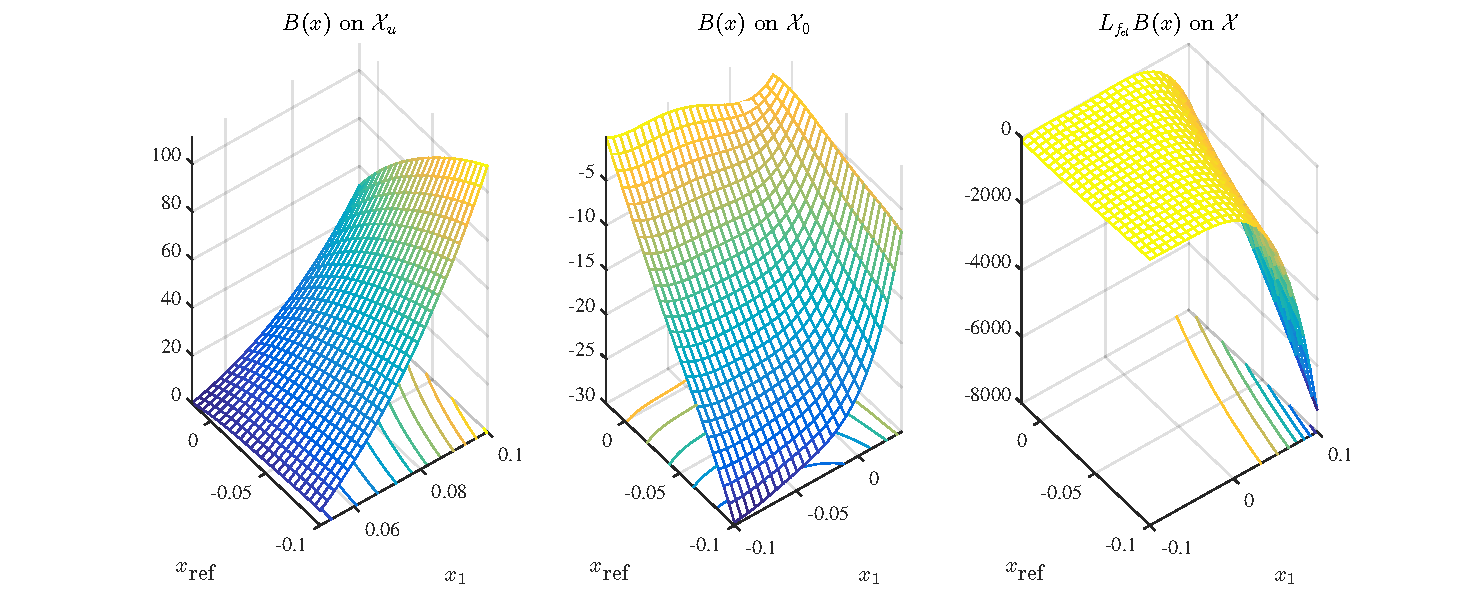
\includegraphics[width=\textwidth]{1storder_withRef.pdf}
\caption{Barrier certificate of degree [0:6], all \gls{sos} polynomials of (monomial) degree [0:2], $\bar{\epsilon}=0.1$, $\Delta=0.015$ and gain $\textbf{K}=0.2$. The solution is found for an interval of references $\mathcal{X}=\{x_\text{ref}[-0.1,0.017] \}$, with \texttt{feasratio=0.9888} and \texttt{Residual norm=3.5e-4}. The plots can be generated by running the script \texttt{1storder\_withRef.m} such that a custom 3D rotation is possible (located in appendix \ref{app:sos_refinterval} under the path \texttt{matlab\_scripts/sostools/1storder\_withRef}).}
\label{fig:1storder_withRef}
\end{figure}

%Note from \autoref{fig:1D_1stordersys_withRef_k02_B6_q2_e01} how the initial expected analysis complies with the actual outcome. Starting from $B(\textbf{x})$ on $\mathcal{X}_u$ it is seen how $B(\textbf{x})>0 \,\,\forall \,x_1 \in [0.05,0.1]$ and $B(\textbf{x})>0 \,\,\forall \,x_\text{ref} \in [0.017,0.1]$ (the reference interval is lower than expected though). Thi

%\begin{figure}[htbp]
%\centering
%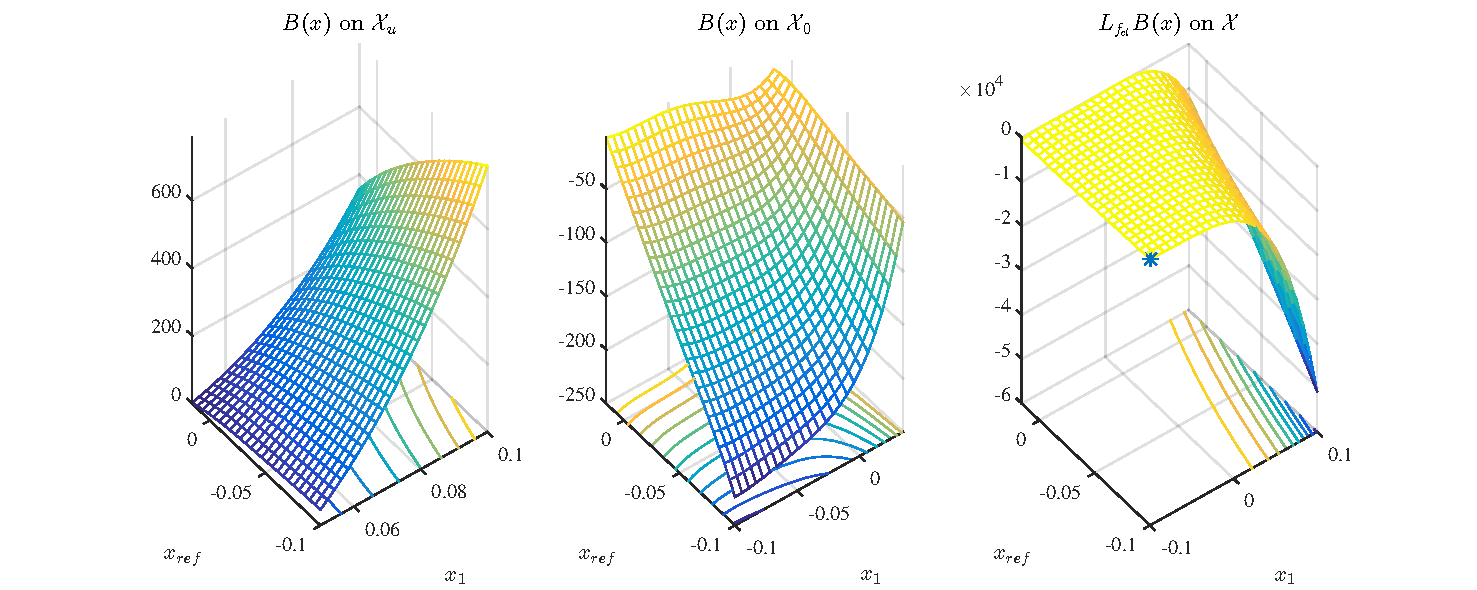
\includegraphics[width=\textwidth]{1D_1stordersys_withRef_k02_B6_q4_e1.pdf}
%\caption{Barrier certificate of degree [0:6], all \gls{sos} polynomials of degree [0:4], $\bar{\epsilon}=1$, $\Delta=0.015$ and gain $\textbf{K}=0.2$ allows an interval of references [-0.1,0.016], with \texttt{feasratio=1.0134} and \texttt{Residual norm=1.6e-3}.}
%\label{fig:1D_1stordersys_withRef_k02_B6_q4_e1}
%\end{figure}


%Testing with controller k=9 as in the initial design. As the zero reference has proven to point of origin is to test with references in a small interval around zero. $\bar{\epsilon}=0.001$ as before but the safety distance $\Delta$ is increased from 0.001 to 0.002. q degrees 0:4
%
%B degree 0:6 -- ok in interval +-1cm, feas ratio 0.9657, numerr 0, resnorm 6.7e-6. expanding downwards, for -3cm feas ratio 0.8727, to -4cm feasratio 0.9342, for -5 feasratio 0.9321, for -6cm feasratio 0.9579, -10, 1.5cm feasr 0.8377, not workin to 2cm, because the Q not working is that for Xu try to increase $\bar{\epsilon}$ and because numerr is 1 (not workin) also increasing $\Delta$ (also not working). Back to $\bar{\epsilon}=0.001$, $\Delta=0.001$. ok with 1.7cm feasr 0.8259 numerr 0 resnorm 0.00064404, works with 2cm feasr 0.6538 numerr 0 resnorm 0.00087217, not working with 2.5cm (or back down to 2.1cm) ---------- increase $\bar{\epsilon}=1$, $\Delta=0.01$ does not work at max -5cm, increase $\Delta=0.02$ works for max -5cm but not for -1cm (and still not working if decreasing $\bar{\epsilon}=0.1$), works for $\bar{\epsilon}=0.01$ feasr 0.9505 numerr 1 resnorm 8.2627e-5, this also works for rmax 1cm feasr 0.9486 numerr 1 resnorm 0.00056789, but not working at 2cm (and still not when decreasing $\Delta=0.01$ or to $\Delta=0.001$)
%
%
%B degree 0:4 -- interval -6, 1cm feas ratio 0.8694, to -7cm feasr 0.9270, -8cm feasr 0.8763 resnorm 0.00027269, -9cm feasr 0.8763, -10cm feasr 0.8255 resnorm 0.00068869, not working with -10, 2cm or with -10,1.5cm, but works with 1.2cm feasr 0.7455 numerr 0 resnorm 0.00060655 "run into numerical problems" (increasing qs to 0:6 still not working with 1.3cm), increasing $\bar{\epsilon}=0.01$ because of numerical problems and resnorm but not working with 1.2cm (also not working when increasing $\Delta=0.01$), but with this delta it works at 0.5cm feasr 0.9030 numerr 1 resnorm 0.0003211, then decreasing delta back not working
%
%try to increase the degree of B and qs drastically, but feasratio becomes negative and Q1 cannot be found (it also takes very long to compute), primal infeasible. Decreasing degrees to B 0:8 and qs 0:6 and $\bar{\epsilon}=0.001$, $\Delta=0.001$ solution found for -10,1.5cm feasr 0.8754, however decreasing degree of qs to 0:4 increases feasr to 0.9458, lowering B to 0:6 feasr 0.8865
%
%or decreasing the region $\mathcal{X}_0$
%
%
%=========================================
%
%with K=0.2, qs 0:4, B 0:6, $\Delta=0.001$, $\bar{\epsilon}=0.001$
%
%-10cm to 2cm: feasr 0.7909 numerr 0, resnorm 0.00011224, not working for 3cm, works for 2.5cm feasr 0.8205 numerr 0 resnorm 0.00031701, and 2.7cm feasr 0.8461 numerr 0, resnorm 0.00021563, not working for 2.8cm, increase $\Delta=0.005$ at 2.2cm works feasr 0.8437 numerr 0 resnorm 9.3091e-5, not working at 2.7cm, also not when decreasing $\Delta=0.0001$, but works at $\Delta=0.0008$ with feasr 0.7027
%
%increase $\bar{\epsilon}=0.01$ ($\Delta=0.001$) not working for 2.7cm, 2.5cm, 2.3cm 2.1cm, works with 1.9cm feasr 0.9116 numerr 1 resnorm 0.00037474, increase $\Delta=0.01$ feasr 0.8619 numerr 0 resnorm 0.00027732
%
%increase $\bar{\epsilon}=0.1$ not working at 1.9cm ($\Delta=0.01$), works at 1.7cm feasr 0.9476 numerr 1 resnorm 0.00037428, decreasing $\Delta=0.001$ not working but works at $\Delta=0.005$ feasr 0.9245 numerr 1 resnorm 0.0005283, for $\Delta=0.015$ works at 1.8cm feasr 0.8212 numerr 0 resnorm 0.00015046, not working at 2cm, but works when decreasing $\Delta=0.01$ works feasr 0.8514 numerr 0 resnorm 0.00043032, not working for 2.2cm (also not when decreasing $\Delta=0.001$ or $\Delta=0.005$,
%$\bar{\epsilon}=0.1$ with $\Delta=0.015$ works at 1.6cm feasr 1.0067 numerr 1 resnorm 0.00014081, not working at 1.8cm
%
%increase $\bar{\epsilon}=1$ not working (for $\Delta=0.005$ at 1.7cm), increase $\Delta=0.01$ not working, down to 1.5cm not working, 1cm not working, increase $\Delta=0.02$ works feasr 0.9683 numerr 1 resnorm 0.0015249, this also works for 1.5cm feasr 1.0014 numerr 1 resnorm 0.00093821, not working at 2cm, decrease $\Delta=0.015$ still not working, or at 1.7cm, works at 1.6cm feasr 1.0134 numerr 1 resnorm 0.0016455, increasing $\Delta=0.02$ not working, or at $\Delta=0.01$

\vspace{-2mm}
It can be concluded that this approach to determining for which references system safety can be guaranteed is not ideal. The tests conducted are not exhaustive, as the possibilities of combining parameter values are vast. This also means that it is highly possible that a "better" barrier certificate can be found certifying safety for a wider range of references without compromising on the feasibility ratio.
In order to decrease the number of parameters, a different approach is used in the following.

\subsection{Considering the Error as the Independent Variable}\label{sec:sos_1storder_error}

As it is seen from \autoref{tab:sostools_varying_param} there are many tuning parameters when searching for a barrier certificate in SOSTOOLS, and iteratively finding a combination giving as large an interval of allowed references outside $\mathcal{X}_u$ as possible can be a long process. 
In the previous section a barrier certificate was found validating the system for references in the interval $x_\text{ref}\in [-0.1,0.017]$\,m, i.e. references up to a distance of 3.3\,cm from the unsafe set, $\mathcal{X}_u=\{x_1\in[0.05,0.1]\}$\, (see \autoref{fig:sos_slide}). 
%Recall the system:
%\begin{flalign*}
%\dot{x} = \underbrace{(\textbf{A} - \textbf{B}\textbf{K})}_{-\tau^{-1}(\textbf{K}+1)} x + \underbrace{\textbf{B}\bar{\textbf{N}}}_{\tau^{-1}(\textbf{K}+1)} x_\text{ref} \kk \Leftrightarrow \kk \dot{x} = \tau^{-1}(\textbf{K}+1)\underbrace{(x_\text{ref} - x)}_{x_\text{err}}
%\end{flalign*}

A different approach is now used in order to validate system safety for references closer to the unsafe set. 
Instead of formulating the barrier certificate in terms of the robot position and the position reference as in \autoref{eq:sos_firstorder}, the dimensionality of the problem can be reduced  through a coordinate shift to the error state as seen in \autoref{fig:sos_error_2d}, the error being: % it can plainly be formulated as the error between the two:
\vspace{-3mm}
\begin{equation*}
x_\text{err}=x_\text{ref}-x_1
\end{equation*}

\vspace{-5mm}
giving the error dynamics
\vspace{-3mm}
\begin{align}
\dot{x}_\text{err} = -\dot{x} &= -\tau^{-1}(\mathbf{K}+1)(x_\text{ref}-x_1) \nonumber\\
&= -\tau^{-1}(\mathbf{K}+1)x_\text{err}
\end{align}

\vspace{-2mm}
Now safety can  be tested for relative positions instead of absolute.

\subsubsection{Relating the Error Space Sets to the Sets for Absolute Position}
 
\vspace{-2mm}
%It is still assumed that any reference given is given outside the unsafe area, which according to \autoref{tab:intervals} is the absolute slide positions $\mathcal{X}_u=\{x_1\in[0.05,0.1]\}$, and it is still the goal to determine how close to the unsafe set references can be given while still guaranteeing safety.
%The error will be negative when the end effector is above the reference, and 
As seen from \autoref{fig:sos_slide}, the unsafe region is the upper part of the interval $\mathcal{X}$, which means that for references given outside the unsafe set, unsafety of the system will only occur if the robot end effector position is above the reference, corresponding to a negative error. This is illustrated in \autoref{fig:sos_delta_error}.
Hence it is required to restrict the error in the negative direction to some value -\gls{deltaerr}, thus restricting the upper value of allowed (safe) references to a distance $\delta_\text{err}$ from the unsafe region, as sketched in \autoref{fig:sos_errorref_1d_new}. %corresponding to restricting how much the end effector position is allowed to be above (more positive than) the reference. 

%If a reference is given at a distance $\delta_\text{err}$ from the unsafe region starting at 5\,cm, it is required that the error does not exceed $-\delta_\text{err}$ in the negative direction. This is illustrated in \autoref{fig:sos_error_2d}. Thus testing how large an interval of allowed references can be given with guaranteed system safety, corresponds to testing how small an (absolute) value of $-\delta_\text{err}$ outlining the unsafe region of the error state system, for which safety can be guaranteed. This is illustrated in \autoref{fig:sos_error_1d}.



\begin{figure}[H]
\centering
\subbottom[]{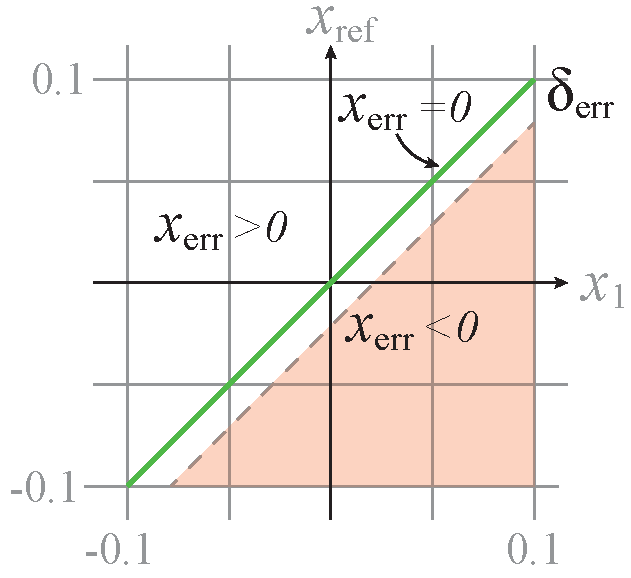
\includegraphics[width=0.3\textwidth]{sos_error_2d.pdf}\label{fig:sos_error_2d}}%
\hspace{3mm}
\subbottom[]{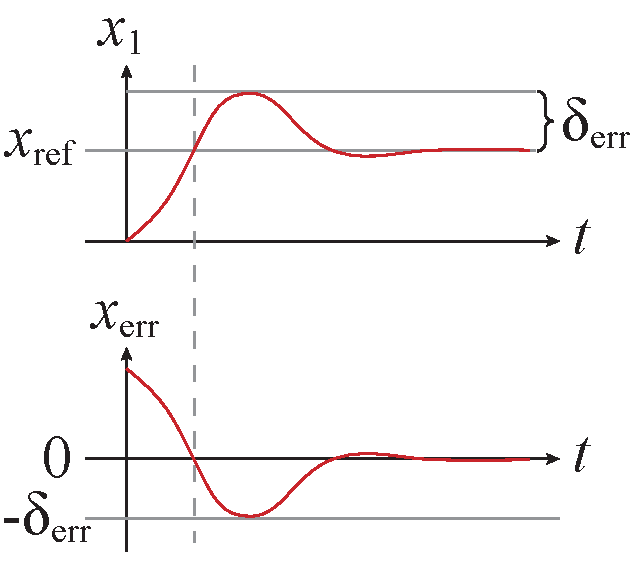
\includegraphics[width=0.3\textwidth]{sos_delta_error.pdf}\label{fig:sos_delta_error}}%
\hspace{3mm}
\subbottom[]{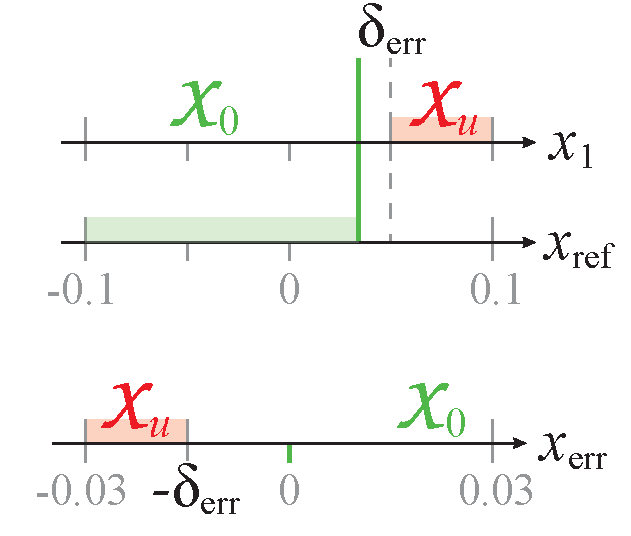
\includegraphics[width=0.3\textwidth]{sos_errorref_1d_new.pdf}\label{fig:sos_errorref_1d_new}}%
\caption{If the error is certified to stay above the value -$\delta_\text{err}$, system safety is guaranteed for all references up to a safety distance of $\delta_\text{err}$ from the unsafe set.}
	\label{fig:sets_error}
\end{figure}

When restricting the error to a lower limit -$\delta_\text{err}$, this restriction corresponds to not allowing the end effector position more than the distance $\delta_\text{err}$ above the reference anywhere outside the unsafe region. However, if a barrier certificate can be found for the error state system with unsafe set being values below -$\delta_\text{err}$, this means that safety of the system in \autoref{eq:sos_firstorder} can be guaranteed for references up to  the distance $\delta_\text{err}$ from the unsafe region.

%this is in principle done for any reference, thus if a reference is given far away from the unsafe area, the end effector is still not allowed to be more than the small distance $\delta_\text{err}$ above the reference. 

%In the error space this means that the error must not go below $-\delta_\text{err}$. If a barrier certificate can be found for unsafe errors of $-\delta_\text{err}$ and below ($\mathcal{X}_u=\{x_\text{err}\in [-??,-\delta_\text{err}]\}$), it can be guaranteed that the robot position will never be more than a distance $\delta_\text{err}$ above the reference, and hence it is verified that references can be given as long as the reference is at least a distance $\delta_\text{err}$ from the unsafe set.

The system equation in \autoref{eq:sos_firstorder} is tested and known to be valid for small steps of approximately 5\,mm, thus the set to be considered in the error state space is chosen to $\pm 3$\,cm. This gives the set definitions for the error state system:
\vspace{-3mm}
\begin{itemize}
\itemsep-0.7mm
\item The set considered is well over the usual reference step size of approximately 5\,mm, $\mathcal{X}=\{x_\text{err}\in[-0.03,0.03] \}$.
\item The unsafe set includes values below -$\delta_\text{err}$, $\mathcal{X}_u=\{x_\text{err}\in [-0.03,-\delta_\text{err}] \}$.
\item The safe set is a distance $\Delta$ from the unsafe set, where $\Delta<\delta_\text{err}$ such that the safe set will include $x_\text{err}=0$, $\mathcal{X}_0=\{x_\text{err}\in [-\delta_\text{err}+\Delta,0.03] \}$.
\end{itemize}

%Due to the underlying low-level controllers in the system (see \autoref{fig:overview}), the system equation in \autoref{eq:sos_firstorder} is only valid for small steps of less than 3\,cm. Therefore the tests on the error state system in SOSTOOLS are made on a set $\mathcal{X}=\{x_\text{err}\in[-0.03,0.03] \}$, thus testing for how small a value $\delta_\text{err}$ for which a solution can be found when the unsafe set is $\mathcal{X}_u=\{x_\text{err}\in[-0.03,-\delta_\text{err}] \}$, as illustrated in \autoref{fig:sos_errorref_1d}. 
If a valid solution can be found, it will certify that steps in positive direction (upwards) of 3\,cm is acceptable, and will never yield an error below $-\delta_\text{err}$, and that references can safely be given as long as they have a distance of at least $\delta_\text{err}$ to the unsafe positions, hence certifying safety of the system: %i.e. safe references are references below 5\,cm $-\delta_\text{err}$. For references below the end effector position no barrier certificate is needed, although the certificate found does allow steps in downwards direction of up to $\delta_\text{err}$. \textcolor{red}{Er ikke sikker p\aa  det giver mening med stepst\o rrelser, er det steady-state fejlen vi ser p\aa ?}
\vspace{-3mm}
\begin{itemize}
	\itemsep-0.7mm
	\item The set considered is the set described in \autoref{fig:sos_slide}, $\mathcal{X}=\{x_1\in[-0.1,0.1] \}$.
	\item The unsafe set is also seen in \autoref{fig:sos_slide}, $\mathcal{X}_u=\{x_1\in [0.05,0.1] \}$.
	\item The safe set for the references is $\mathcal{X}_0=\{x_\text{ref}\in [-0.1,0.05-\delta_\text{err}] \}$ ensuring that $\mathcal{X}_0\subseteq\mathcal{X}\setminus\mathcal{X}_u$.
\end{itemize}

\subsubsection{Results and Conclusions}

\vspace{-2mm}
The parameters $\bar{\epsilon}$, $\Delta$, $\delta_\text{err}$, and the degree of the \gls{sos} polynomials $q_j$ and the polynomial $B(x_\text{err})$, are tweaked to find the smallest possible value of $\delta_\text{err}$ yielding a valid solution.
The MATLAB implementation of this approach can be found in appendix \ref{app:sos_refinterval} and in \autoref{app:cd} under the path \texttt{matlab\_scripts/ sostools/1storder\_error.m}.
The findings conform with the conclusions presented in \autoref{tab:sostools_varying_param}, with the additional conclusions listed in \autoref{tab:sostools_varying_param_error}.

 





\begin{table}[htbp]
\begin{tabularx}{\textwidth}{l X}
\rowcolor{HeaderBlue}
\textbf{Parameter} & \textbf{Effect of variation}\\
deg$(B)$ & In general the residual norm is lower when testing for higher degrees of $B(x_\text{err})$ ([0:6] compared to [0:4]).\\
\rowcolor{textBlue}
deg$(q_j)$ & Increasing the degree of the \gls{sos} polynomials (monomial degrees [0:4] compared to [0:2]) generally increases the residual norm. Having different degrees for the different \gls{sos} polynomials also generally increases the residual norm.\\
$\bar{\epsilon}$ & Increasing $\bar{\epsilon}$ in general increases the residual norm of the solution. \\
\rowcolor{textBlue}
$\Delta$ & Decreasing $\Delta$ too much will preclude a solution to be found, otherwise $\Delta$ does not have much influence on the solution.\\
\textbf{K} & Lowering the gain of the controller decreases the residual norm of the solution.\\
\rowcolor{textBlue}
$\delta_\text{err}$ & Decreasing $\delta_\text{err}$ increases the residual norm of the solution. %No solutions could be found for $\delta_\text{err}<9$\,mm.
\end{tabularx}
\caption{Effect of varying different parameters in the \gls{sos} program. Results are only included for solutions where all inequalities were verified to be \gls{sos}.}
\label{tab:sostools_varying_param_error}
\end{table}

%systemet har underliggende controllere der gør at systemmodellen kun gælder hvis der gives små steps i reference, derfor er der ingen grund til at define et rum X i errorspace der er større til hver side end de step der kan gives

\begin{table}[htbp]
\begin{tabularx}{\textwidth}{l X}
		\rowcolor{HeaderBlue}
		\textbf{Choice} & \textbf{Reason}\\
		deg$(B)=$ [0:6] & Increasing the degree of the barrier certificate from [0:4] to [0:6] does not change the curve much on the interval $\mathcal{X}$, while it does lower the residual norm an order.\\
		\rowcolor{textBlue}
		deg$(q_j)=$ [0:4] & The degree of the \gls{sos} polynomials are chosen as low as possible allowing a solution to be found with the remaining parameters.\\
		$\bar{\epsilon}=1e$-2 & Increasing  $\bar{\epsilon}$ by an order of magnitude scales up the barrier certificate approximately ten times in value, but also increases  the residual norm approximately an order of magnitude. A compromise is made choosing a scaling of $B(x_\text{err})$ yielding neither very small nor very large values of $B(x_\text{err})$ on the set $\mathcal{X}$, still giving a solution with relatively low residual norm. \\
		\rowcolor{textBlue}
		$\Delta=4e$-3 & The value of $\Delta$ is desired as low as possible, and at least lower than $\delta_\text{err}$ (such that the safe set will include $x_\text{err}=0$). The lowest value yielding a solution is chosen.\\
		$\textbf{K}=0.2$ & A low gain is chosen identical to the choice in \autoref{sec:sos_1storder_references}, as implementable gains are ascertained to be of this order.\\
		\rowcolor{textBlue}
		$\delta_\text{err}=9e$-3 & No solutions could be found for $\delta_\text{err}<9$\,mm.
\end{tabularx}
\caption{Chosen value for each of the parameters. The barrier certificate is plotted in \autoref{fig:1D_1stordersys_error_k02_B6_q4_varying_epsilon}. % as the yellow curve, along with scaled certificates found for different values of $\bar{\epsilon}$.
	}
\label{tab:sostools_choice_error}
\end{table}

The choice of parameter values are explained in \autoref{tab:sostools_choice_error} and the barrier certificate is plotted in \autoref{fig:1D_1stordersys_error_k02_B6_q4_varying_epsilon}. % as the yellow curve along with scaled certificates found for different values of $\bar{\epsilon}$. 
It is seen that the barrier certificate is positive on the unsafe region below -9\,mm, i.e.  $\mathcal{X}_u=\{x_\text{err}\in[-0.03,-\delta_\text{err}]\}=\{x_\text{err}\in[-0.03,-0.009]\}$, and nonpositive on the safe region $\mathcal{X}_0=\{x_\text{err}\in[-\delta_\text{err}+\Delta,0.03]\}=\{x_\text{err}\in[-0.005,0.03]\}$, and that its Lie derivative is nonpositive on the entire set $\mathcal{X}=\{x_\text{err} \in[-0.03,0.03] \}$, confirming that it is a valid barrier certificate in accordance with \autoref{def:barrier_certificate}.

Relating this relative position to the absolute positions, this  certificate guarantees  safety for the system in  \autoref{eq:sos_firstorder} with references up until a minimum distance of 9\,mm from the unsafe set in $\mathcal{X}_u=\{x_1\in[0.05,0.1] \}$ (see \autoref{fig:sos_slide}), i.e. system safety is guaranteed for references in the interval $\mathcal{X}_0=\{x_\text{ref}\in[-0.1,0.041] \}$.
Thus, this barrier certificate verifies safety for a considerably less restrictive set of references, as it guarantees safety for references at distances as low as 9\,mm from the unsafe region, compared to the 3.3\,cm found with the approach described in \autoref{sec:sos_1storder_references}.






%\begin{figure}[htbp]
%\centering
%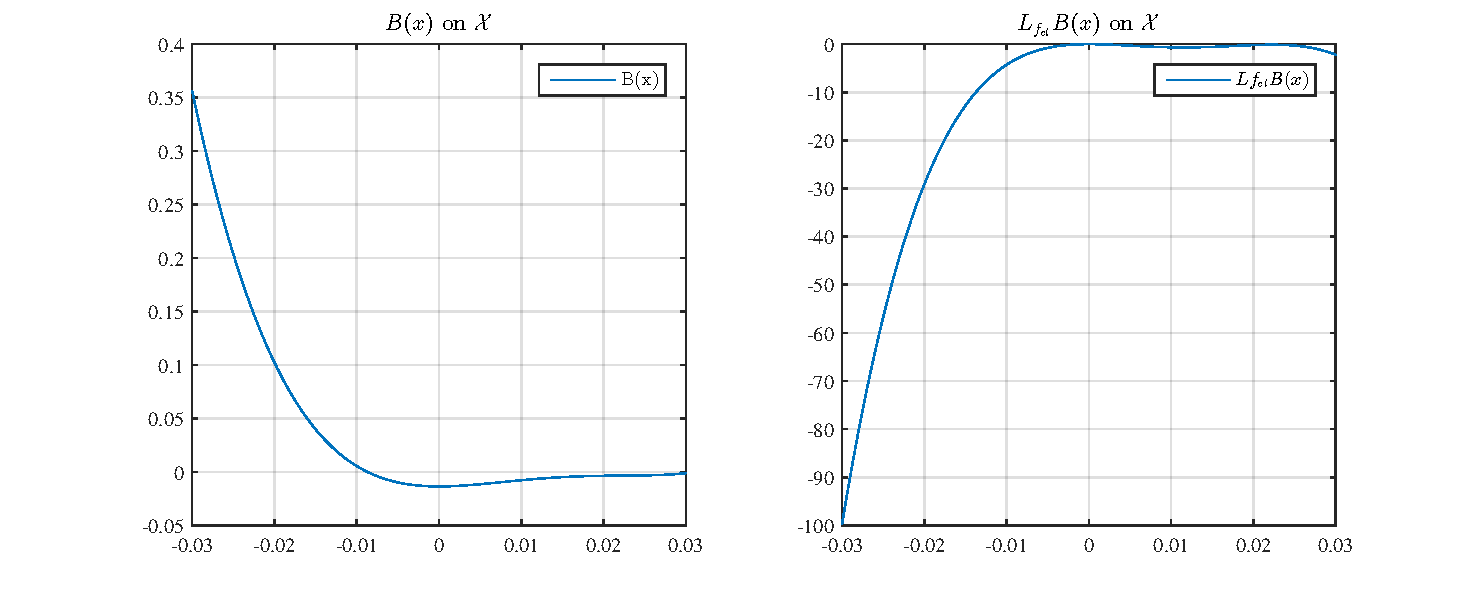
\includegraphics[width=\textwidth]{1D_1stordersys_error_k9_B4_q2_e5-4_d1-2.pdf}
%\caption{Barrier certificate of degree [0:4], all \gls{sos} polynomials of degree [0:2], $\bar{\epsilon}=5e$-4, $\Delta=1e$-2 and gain $\textbf{K}=9$, with \texttt{feasratio=0.9956} and \texttt{Residual norm=4.4e-7}.}
%\label{fig:1D_1stordersys_error_k9_B4_q2_e5-4_d1-2}
%\end{figure}

%\begin{figure}[htbp]
%\centering
%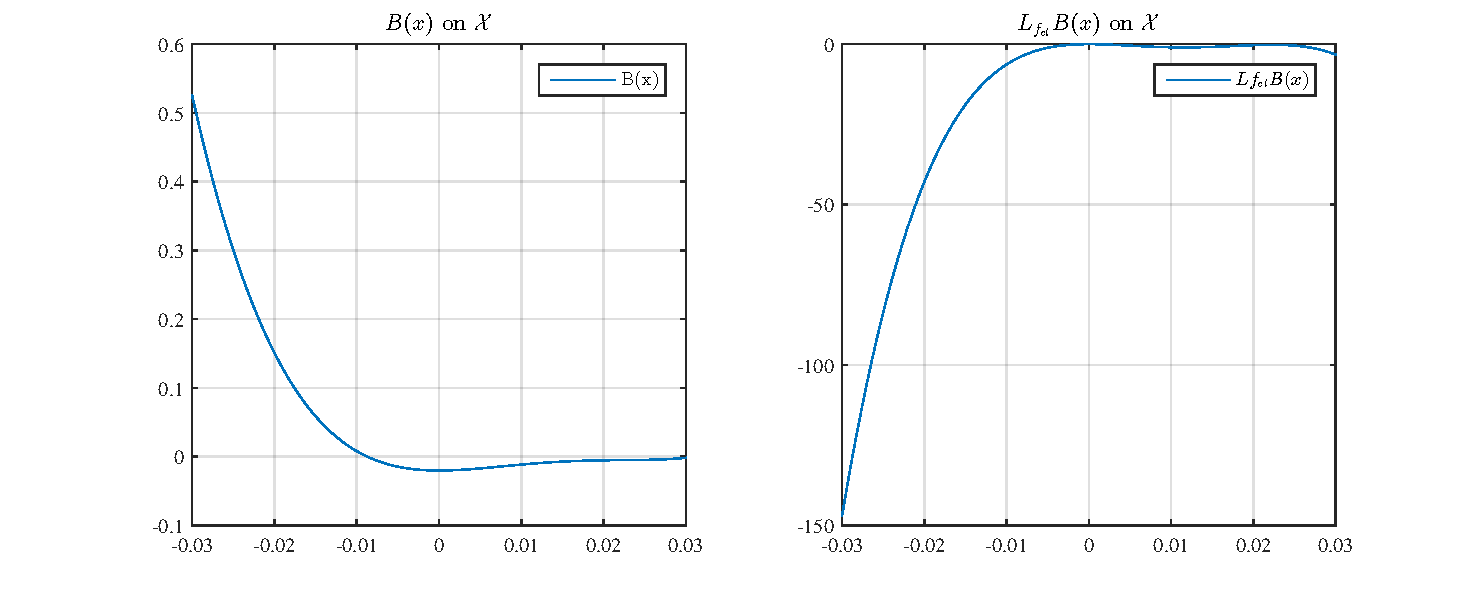
\includegraphics[width=\textwidth]{1D_1stordersys_error_k9_B4_q2_e7-4_d1-3.pdf}
%\caption{Barrier certificate of degree [0:4], all \gls{sos} polynomials of degree [0:2], $\bar{\epsilon}=7e$-4, $\Delta=1e$-3 and gain $\textbf{K}=9$, with \texttt{feasratio=1.0120} and \texttt{Residual norm=3.7e-7}.}
%\label{fig:1D_1stordersys_error_k9_B4_q2_e7-4_d1-3}
%\end{figure}

%\begin{figure}[htbp]
%\centering
%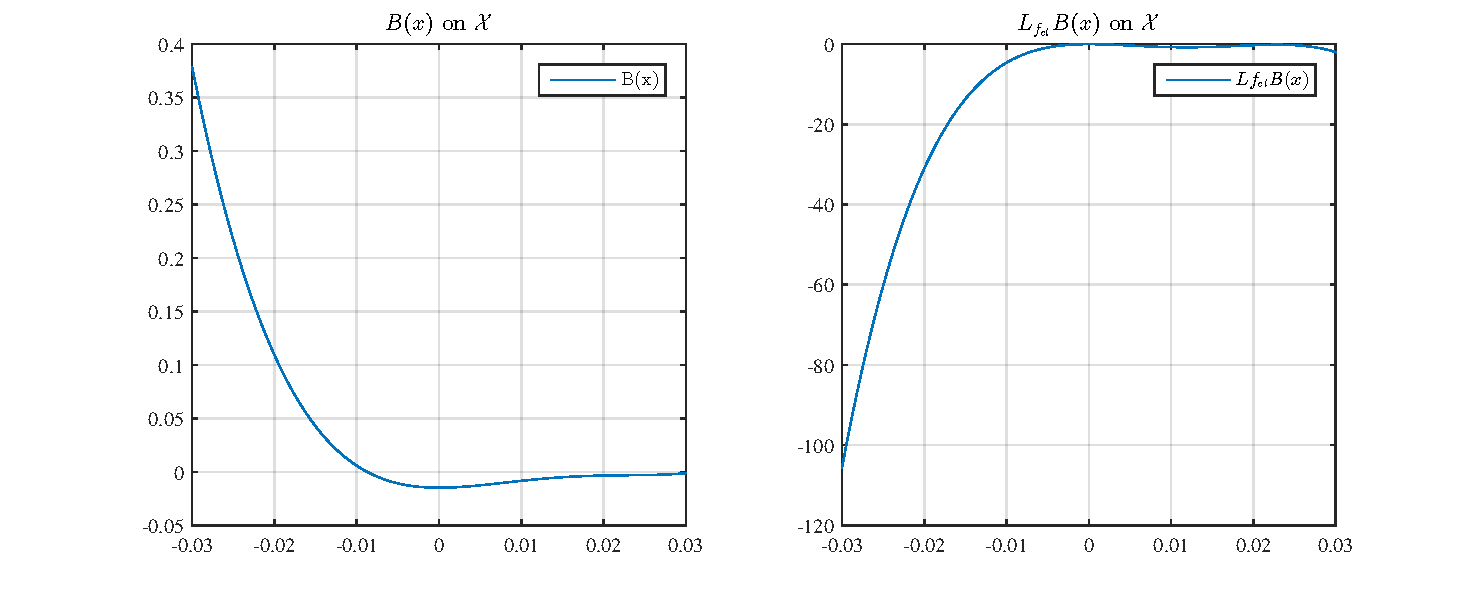
\includegraphics[width=\textwidth]{1D_1stordersys_error_k9_B4_q3_e5-4_d1-2.pdf}
%\caption{Barrier certificate of degree [0:4], all \gls{sos} polynomials of degree [0:3], $\bar{\epsilon}=5e$-4, $\Delta=1e$-2 and gain $\textbf{K}=9$, with \texttt{feasratio=0.8604} and \texttt{Residual norm=1.6e-5}.}
%\label{fig:1D_1stordersys_error_k9_B4_q3_e5-4_d1-2}
%\end{figure}

%\begin{figure}[htbp]
%\centering
%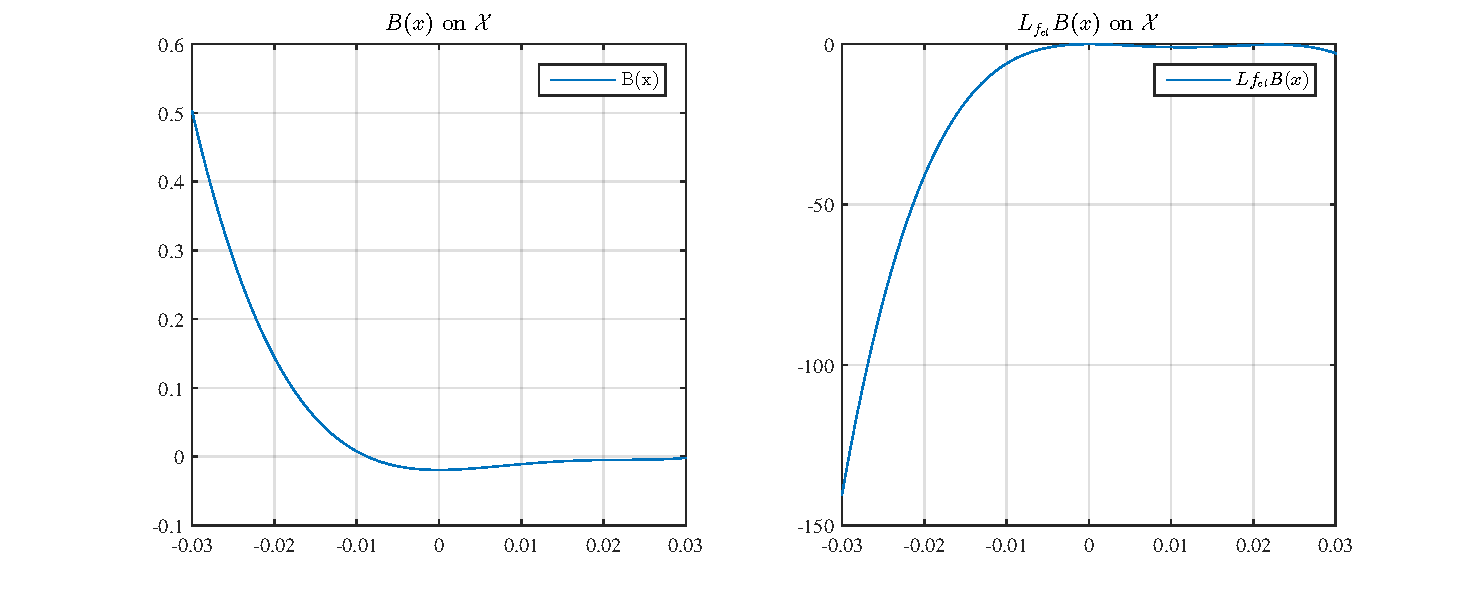
\includegraphics[width=\textwidth]{1D_1stordersys_error_k9_B6_q2_e7-4_d1-3.pdf}
%\caption{Barrier certificate of degree [0:6], all \gls{sos} polynomials of degree [0:2], $\bar{\epsilon}=7e$-4, $\Delta=1e$-3 and gain $\textbf{K}=9$, with \texttt{feasratio=1.0392} and \texttt{Residual norm=4.7e-8}.}
%\label{fig:1D_1stordersys_error_k9_B6_q2_e7-4_d1-3}
%\end{figure}

%\begin{figure}[htbp]
%\centering
%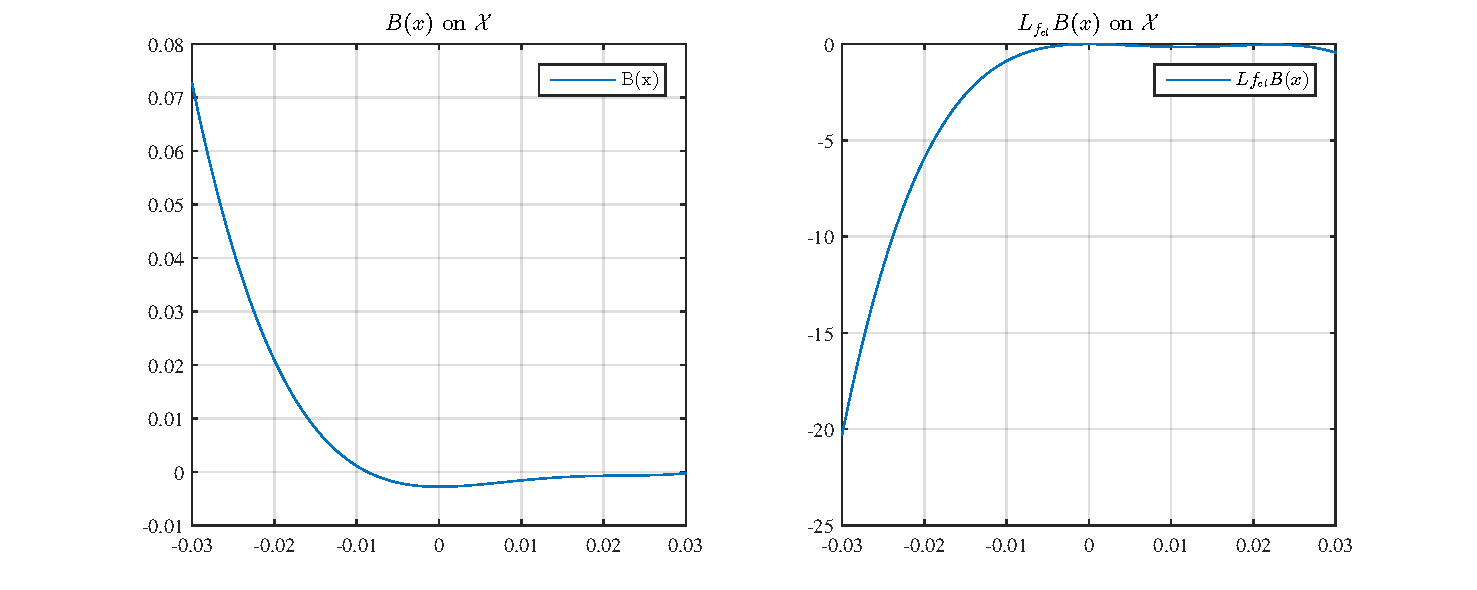
\includegraphics[width=\textwidth]{1D_1stordersys_error_k9_B6_q4_e1-4_d1-3.pdf}
%\caption{Barrier certificate of degree [0:6], all \gls{sos} polynomials of degree [0:4], $\bar{\epsilon}=1e$-4, $\Delta=1e$-3 and gain $\textbf{K}=9$, with \texttt{feasratio=1.027} and \texttt{Residual norm=3.3e-8}.}
%\label{fig:1D_1stordersys_error_k9_B6_q4_e1-4_d1-3}
%\end{figure}

%\begin{figure}[htbp]
%\centering
%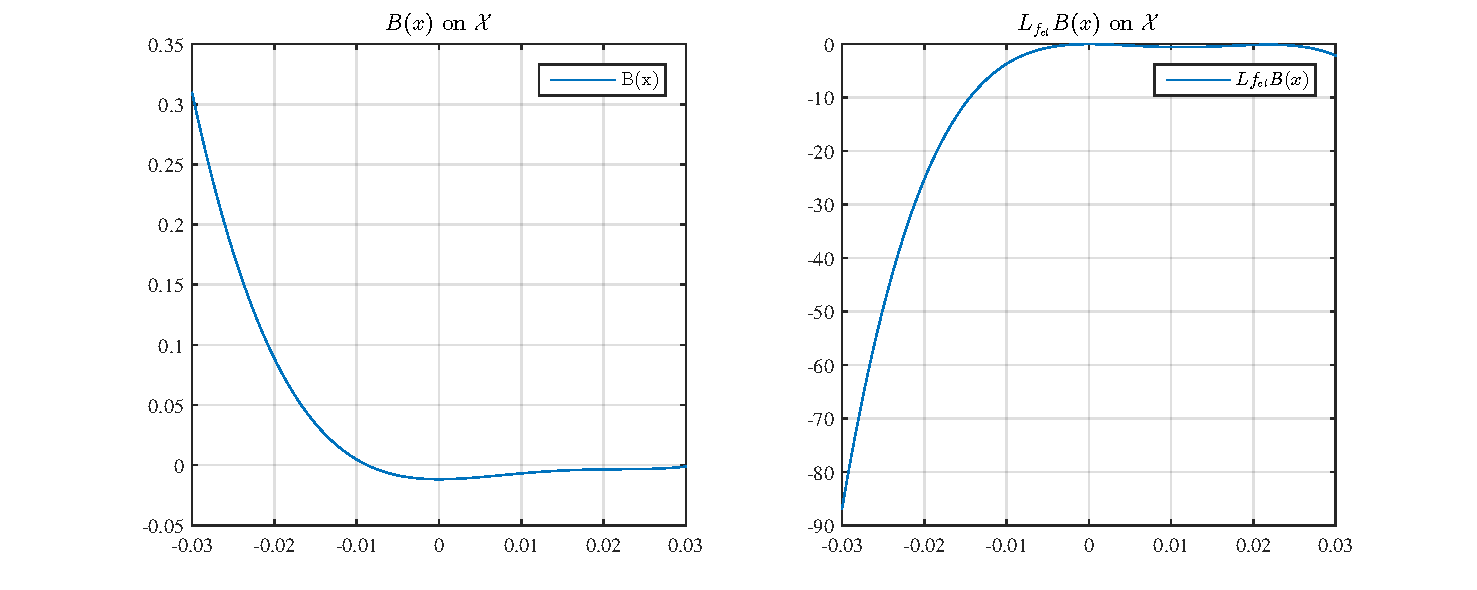
\includegraphics[width=\textwidth]{1D_1stordersys_error_k9_B6_q4_e5-4_d4-3.pdf}
%\caption{Barrier certificate of degree [0:6], all \gls{sos} polynomials of degree [0:4], $\bar{\epsilon}=5e$-4, $\Delta=4e$-3 and gain $\textbf{K}=9$, with \texttt{feasratio=1.0632} and \texttt{Residual norm=8.4e-8}.}
%\label{fig:1D_1stordersys_error_k9_B6_q4_e5-4_d4-3}
%\end{figure}

%\begin{figure}[htbp]
%\centering
%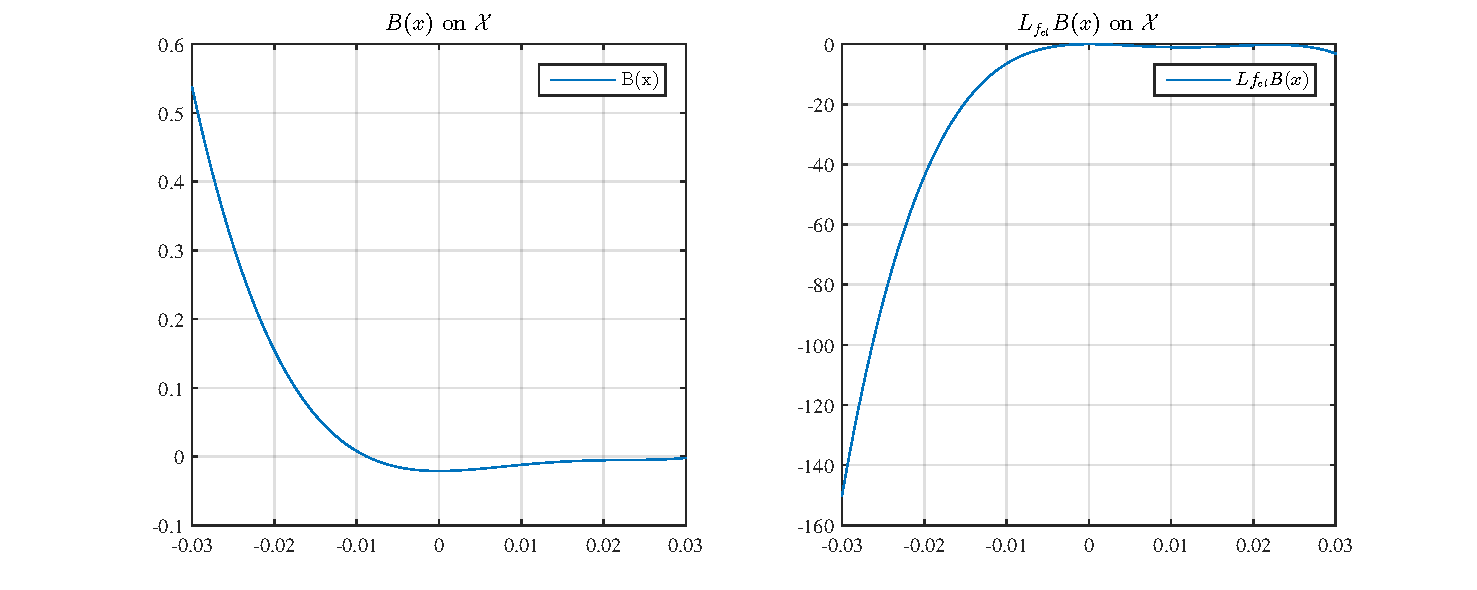
\includegraphics[width=\textwidth]{1D_1stordersys_error_k9_B6_q4_e7-4_d1-3.pdf}
%\caption{Barrier certificate of degree [0:6], all \gls{sos} polynomials of degree [0:4], $\bar{\epsilon}=7e$-4, $\Delta=1e$-3 and gain $\textbf{K}=9$, with \texttt{feasratio=1.0142} and \texttt{Residual norm=1.1e-6}.}
%\label{fig:1D_1stordersys_error_k9_B6_q4_e7-4_d1-3}
%\end{figure}

%\begin{figure}[htbp]
%\centering
%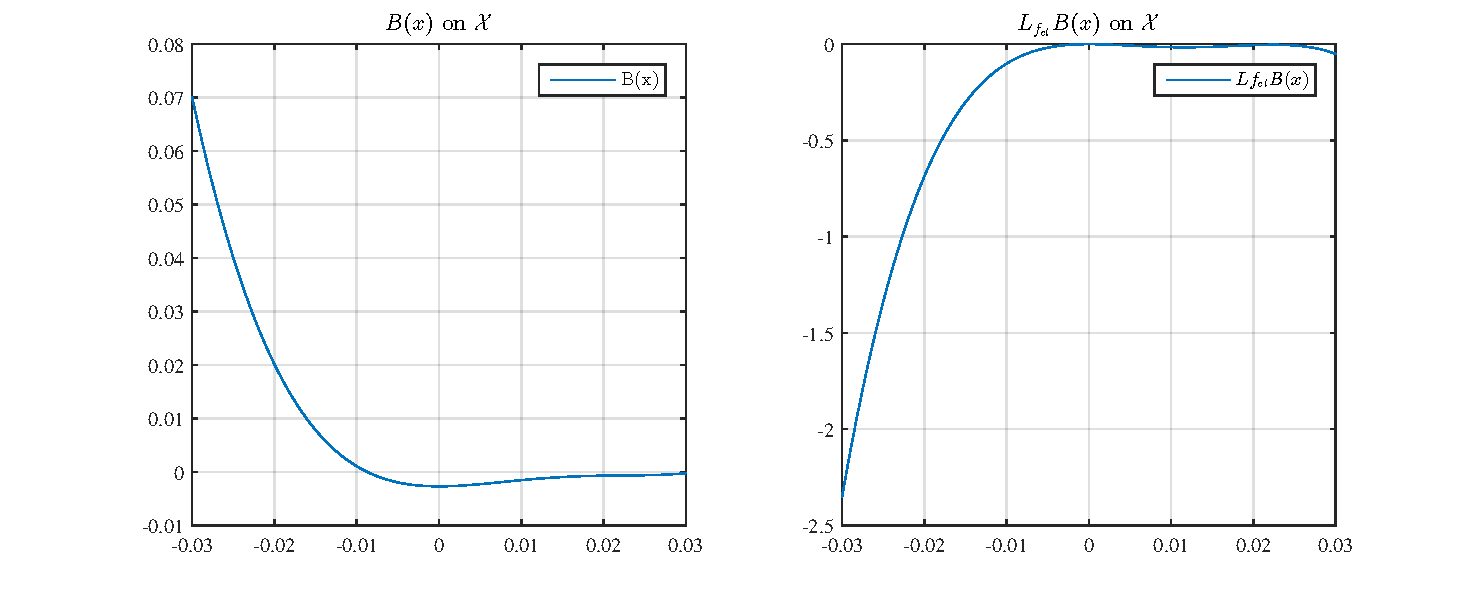
\includegraphics[width=\textwidth]{1D_1stordersys_error_k02_B6_q2_e1-4_d1-3.pdf}
%\caption{Barrier certificate of degree [0:6], all \gls{sos} polynomials of degree [0:2], $\bar{\epsilon}=1e$-4, $\Delta=1e$-3 and gain $\textbf{K}=0.2$, with \texttt{feasratio=1.0539} and \texttt{Residual norm=2.2e-9}.}
%\label{fig:1D_1stordersys_error_k02_B6_q2_e1-4_d1-3}
%\end{figure}

%\begin{figure}[htbp]
%\centering
%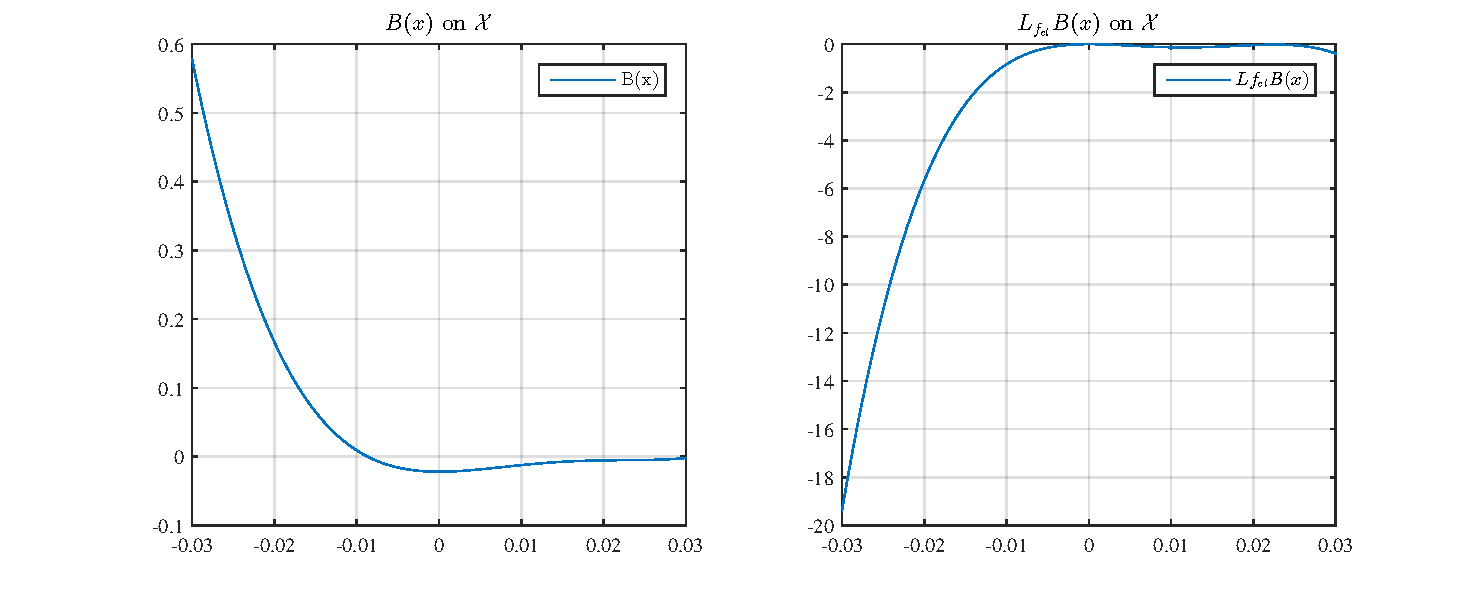
\includegraphics[width=\textwidth]{1D_1stordersys_error_k02_B6_q4_e1-3_d4-3.pdf}
%\caption{Barrier certificate of degree [0:6], all \gls{sos} polynomials of degree [0:4], $\bar{\epsilon}=1e$-3, $\Delta=4e$-3 and gain $\textbf{K}=0.2$, with \texttt{feasratio=1.0495} and \texttt{Residual norm=1.9e-8}.}
%\label{fig:1D_1stordersys_error_k02_B6_q4_e1-3_d4-3}
%\end{figure}


%\begin{figure}[htbp]
%\centering
%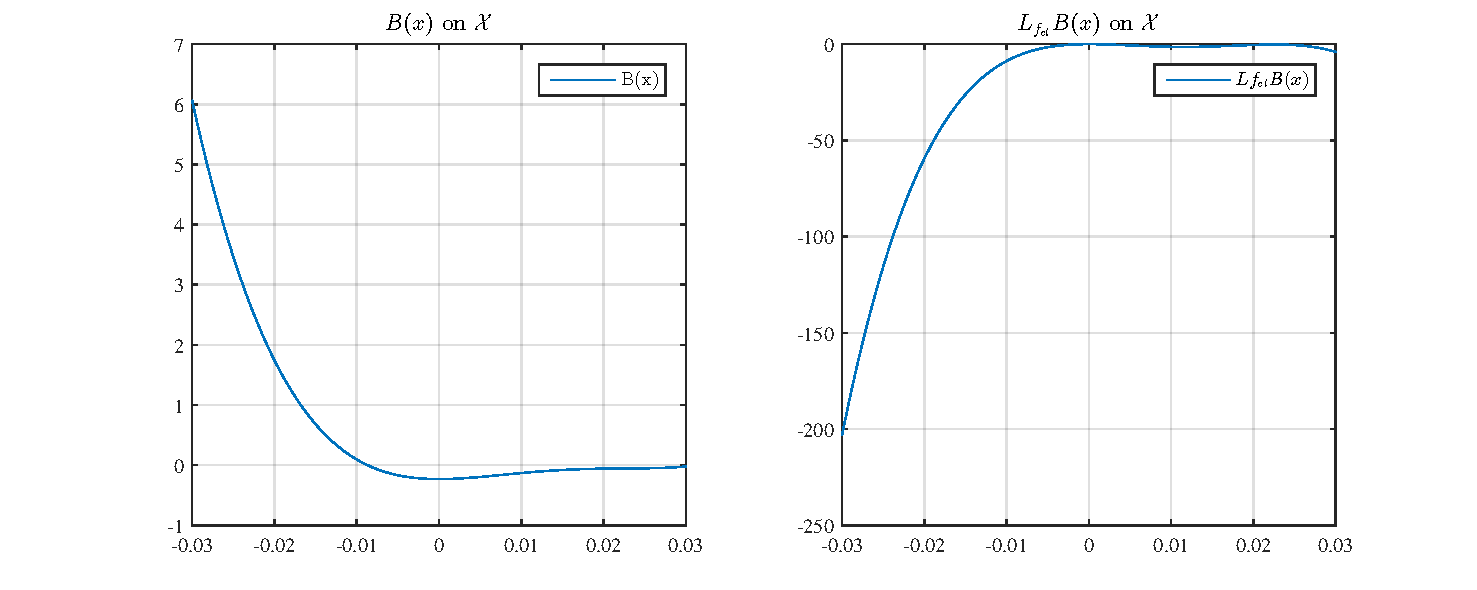
\includegraphics[width=\textwidth]{1D_1stordersys_error_k02_B6_q4_e1-2_d4-3.pdf}
%\caption{Barrier certificate of degree [0:6], all \gls{sos} polynomials of degree [0:4], $\bar{\epsilon}=1e$-2, $\Delta=4e$-3 and gain $\textbf{K}=0.2$, with \texttt{feasratio=1.0262} and \texttt{Residual norm=2.8e-7}.}
%\label{fig:1D_1stordersys_error_k02_B6_q4_e1-2_d4-3}
%\end{figure}


%\begin{figure}[htbp]
%\centering
%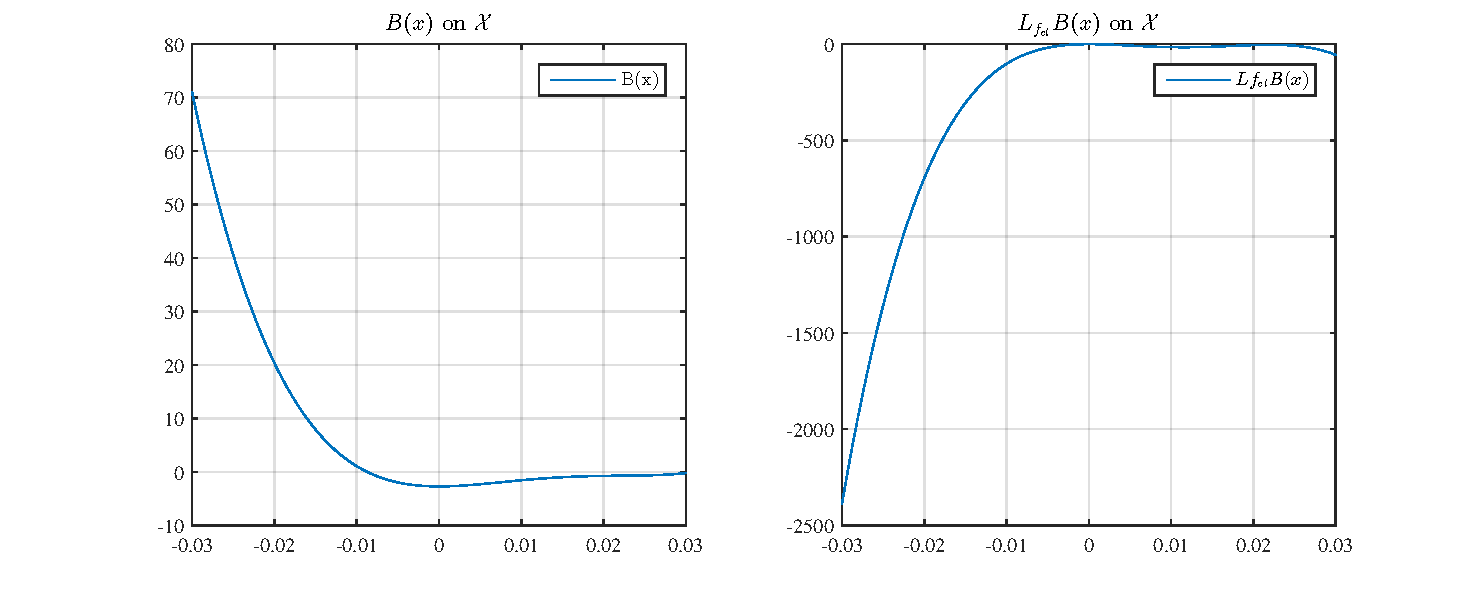
\includegraphics[width=\textwidth]{1D_1stordersys_error_k02_B6_q4_e1-1_d4-3.pdf}
%\caption{Barrier certificate of degree [0:6], all \gls{sos} polynomials of degree [0:4], $\bar{\epsilon}=1e$-1, $\Delta=4e$-3 and gain $\textbf{K}=0.2$, with \texttt{feasratio=1.0298} and \texttt{Residual norm=2.5e-6}.}
%\label{fig:1D_1stordersys_error_k02_B6_q4_e1-1_d4-3}
%\end{figure}

%\begin{figure}[htbp]
%\centering
%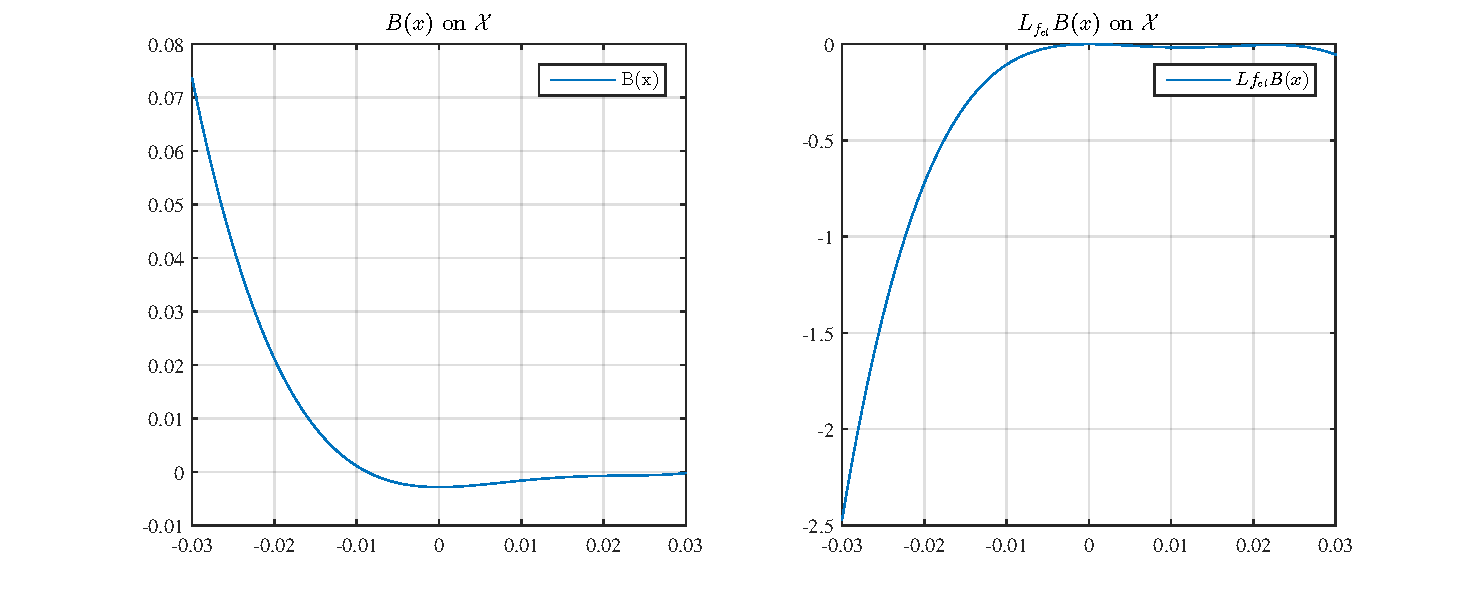
\includegraphics[width=\textwidth]{1D_1stordersys_error_k02_B6_q4_e1-4_d1-3.pdf}
%\caption{Barrier certificate of degree [0:6], all \gls{sos} polynomials of degree [0:4], $\bar{\epsilon}=1e$-4, $\Delta=1e$-3 and gain $\textbf{K}=0.2$, with \texttt{feasratio=0.9664} and \texttt{Residual norm=1.9e-8}.}
%\label{fig:1D_1stordersys_error_k02_B6_q4_e1-4_d1-3}
%\end{figure}

%\begin{figure}[htbp]
%\centering
%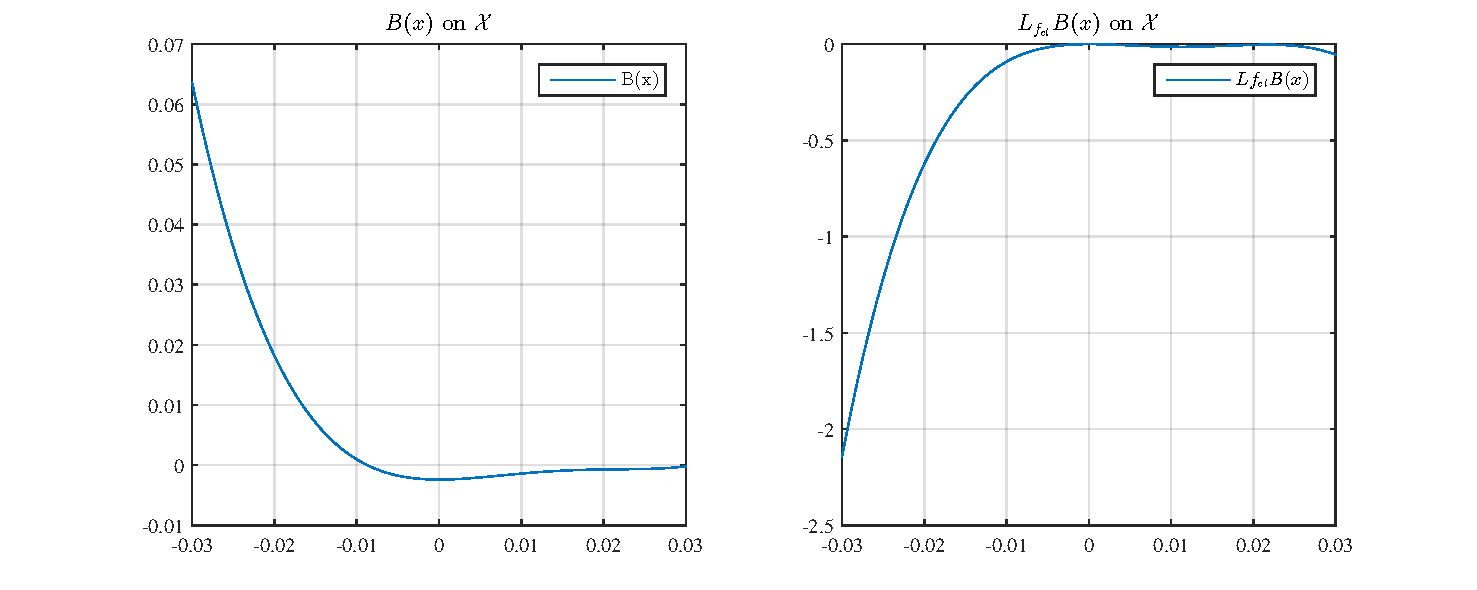
\includegraphics[width=\textwidth]{1D_1stordersys_error_k02_B6_q4_e1-4_d4-3.pdf}
%\caption{Barrier certificate of degree [0:6], all \gls{sos} polynomials of degree [0:4], $\bar{\epsilon}=1e$-4, $\Delta=4e$-3 and gain $\textbf{K}=0.2$, with \texttt{feasratio=1.0096} and \texttt{Residual norm=9.9e-10}.}
%\label{fig:1D_1stordersys_error_k02_B6_q4_e1-4_d4-3}
%\end{figure}

%\begin{figure}[htbp]
%\centering
%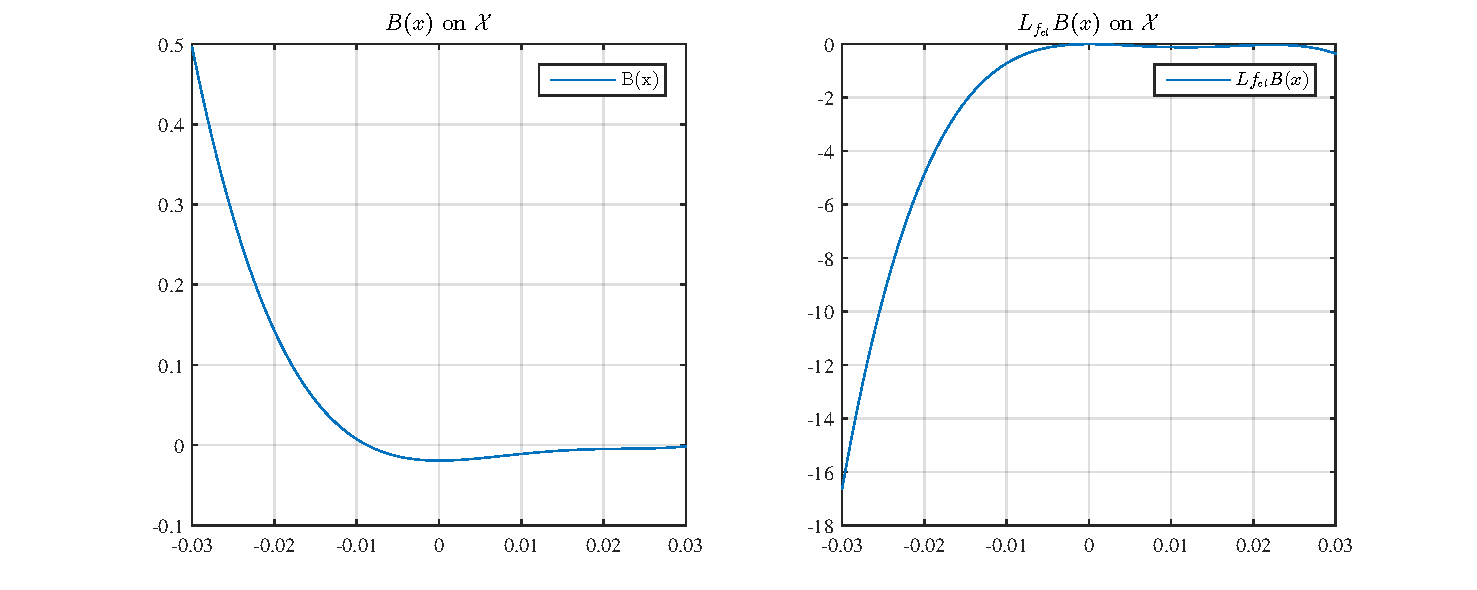
\includegraphics[width=\textwidth]{1D_1stordersys_error_k02_B6_q4_e7-4_d1-3.pdf}
%\caption{Barrier certificate of degree [0:6], all \gls{sos} polynomials of degree [0:4], $\bar{\epsilon}=7e$-4, $\Delta=1e$-3 and gain $\textbf{K}=0.2$, with \texttt{feasratio=0.9988} and \texttt{Residual norm=5.8e-8}.}
%\label{fig:1D_1stordersys_error_k02_B6_q4_e7-4_d1-3}
%\end{figure}

%\begin{figure}[H]
%	\centering
%	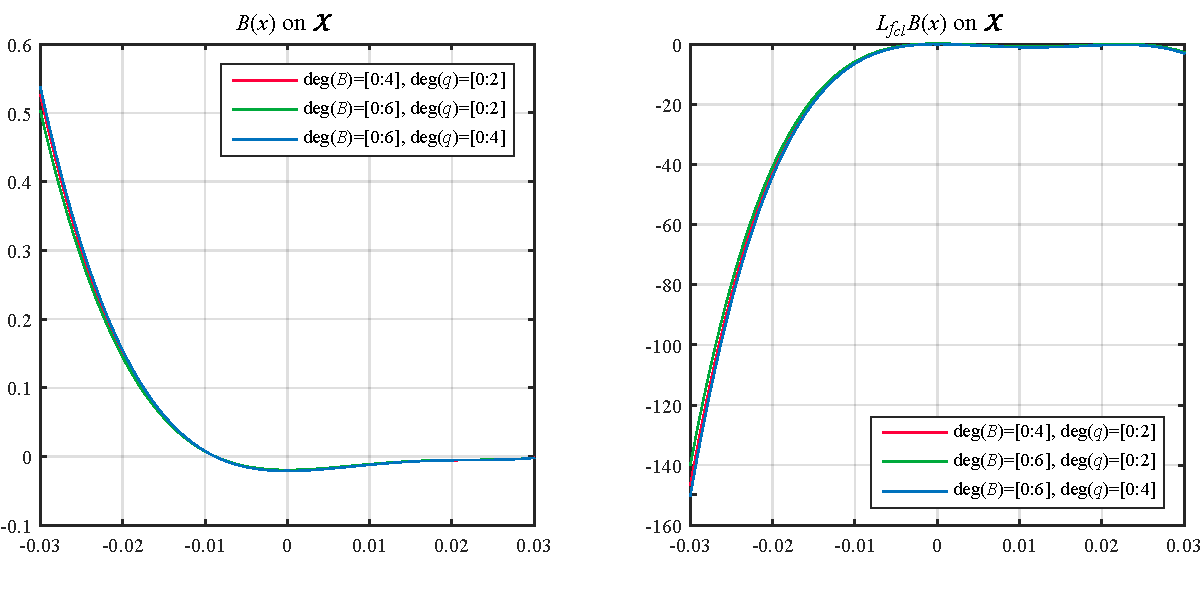
\includegraphics[width=0.9\textwidth]{1D_1stordersys_error_k9_varying_degrees.pdf}
%	\caption{Barrier certificates with $\bar{\epsilon}=7e$-4, $\Delta=1e$-3 and gain $\textbf{K}=9$. Varying the degrees of the barrier certificate and the \gls{sos} polynomials, where deg$(B)=$[0:4] and deg$(q)=$[0:2] gives  \texttt{feasratio=1.0120} and \texttt{Residual norm=3.7e-7}, deg$(B)=$[0:6] and deg$(q)=$[0:2] gives  \texttt{feasratio=1.0392} and \texttt{Residual norm=4.7e-8}, deg$(B)=$[0:6] and deg$(q)=$[0:4] gives \texttt{feasratio=1.0142} and \texttt{Residual norm=1.1e-6}.}
%	\label{fig:1D_1stordersys_error_k9_varying_degrees}
%\end{figure}

\begin{figure}[H]
	\centering
	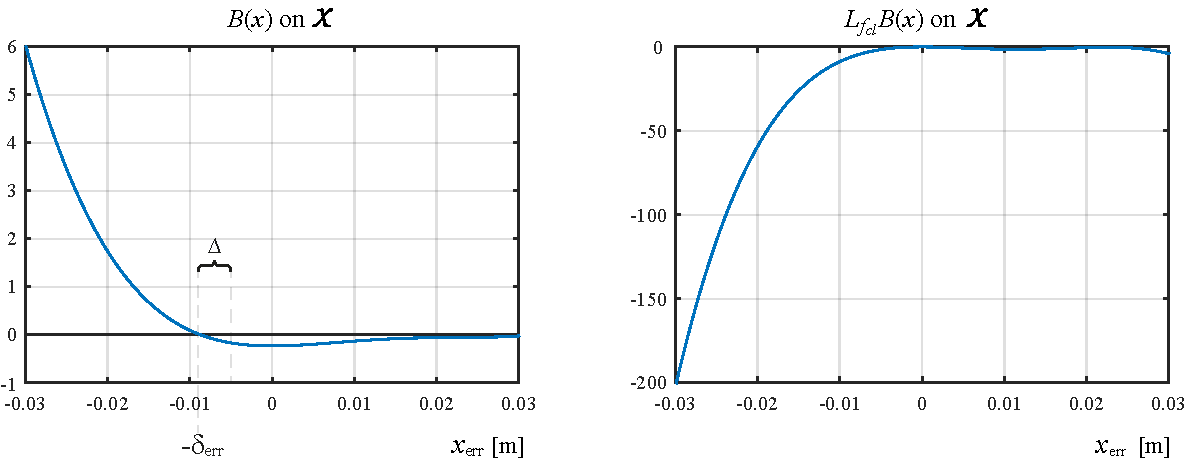
\includegraphics[width=\textwidth]{1D_1stordersys_error_k02_B6_q4_chosen_epsilon.pdf}
	\caption{Barrier certificate of degree [0:6], all \gls{sos} polynomials of degree [0:4], with  $\bar{\epsilon}=1e$-2, $\Delta=4e$-3, $\delta_\text{err}=9e$-3 and gain $\textbf{K}=0.2$. %Varying the value of $\bar{\epsilon}$, where $\bar{\epsilon}=1e$-4 gives \texttt{feasratio=1.0096} and \texttt{Residual norm=9.9e-10}, $\bar{\epsilon}=1e$-3 gives \texttt{feasratio=1.0495} and \texttt{Residual norm=1.9e-8}, $\bar{\epsilon}=1e$-2, gives \texttt{feasratio=1.0262} and \texttt{Residual norm=2.8e-7}, $\bar{\epsilon}=1e$-1 gives \texttt{feasratio=1.0298} and \texttt{Residual norm=2.5e-6}.
	The solution has a \texttt{feasratio=1.0262} and \texttt{Residual norm=2.8e-7}.}
	\label{fig:1D_1stordersys_error_k02_B6_q4_varying_epsilon}
\end{figure}

A corresponding positive value can be found restricting the error in the positive direction hence also restricting how much the end effector position is allowed to be below any reference.  Although this is not tested, it is clear that if a barrier certificate for the error can be found ensuring that the error will stay within the interval $\mathcal{X}_0\subseteq \{x_\text{err}\in[-\delta_\text{err},\delta_\text{err}] \}$ i.e. with unsafe regions on both sides of this interval, this means that for any reference, the end effector position can be guaranteed never to be more than a distance $\delta_\text{err}$ away from the reference. %\textcolor{red}{in steady-state? It cannot say anything about steps that are larger than $\delta_\text{err}$, but maybe we don't care about that?}